% !TEX root = ../thesis.tex

\chapter{Evaluation}
\label{evaluation}

Dieses Kapitel dient der Evaluation der im vorangegangenen Kapitel erläuterten Klassifikationen. Dies geschieht durch verschiedene Evaluationsmetriken, welche in diesem Kapitel vorgestellt werden und auf Werten von sogenannten Konfusionsmatrizen basieren. Zudem umfasst dieses Kapitel eine Erläuterung von Herausforderungen und Limitationen, die im Laufe der Bearbeitung der Arbeit festgestellt worden sind. Abschließen wird dieses Kapitel ein Vergleich der Klassifikatoren zu einer klassischen dateibasierten Methode, welche aus der wissenschaftlichen Literatur entnommen wurde.
\\
\hrule

\section{Herausforderungen und Limitationen}

szz \\
absprechen mit Daniel
...

\section{Vergleich der Klassifikatoren}

Der Vergleich der Klassifikatoren erfolgt unter Zuhilfenahme von Evaluationsmetriken, die im nachfolgenden Abschnitt vorgestellt werden. Die Diskussion der Ergebnisse der Evaluation erfolgt in \hyperref[results]{Abschnitt 5.2.2}.

\subsection{Evaluationsmetriken}
\label{eval-metrics}

Die zum Vergleich der Klassifikatoren erhobenen Evaluationmetriken entstammen dem Themengebiet des Information Retrieval und gelten als Standardmesswerte für ihren Einsatzzweck \cite{Sammut2017}. Der Großteil dieser Metriken lässt sich anhand von Werten einer sogenannten Konfusionsmatrix berechnen und messen allesamt die Performanz der Vorhersagen von Klassifikatoren. Im Falle einer binären Klassifikation, wie in dieser Arbeit, besteht diese Matrix aus vier Gruppen, deren Werte angeben, ob der jeweilige Klassifikator ein Objekt korrekt oder falsch einer der beiden Zielklassen zuordnen konnte \cite{Sammut2017}. Im Zusammenhang mit solchen Matrizen werden die beiden Zielklassen \glqq positiv\grqq{} und \glqq negativ\grqq{} genannt. Für diese Arbeit werden die positive Klasse dem Label \glqq fehlerfrei\grqq und die negative Klasse dem Label \glqq defekt\grqq{} zugeordnet. Die Form einer allgemeinen Konfusionsmatrix ist in \autoref{fig:confu} dargestellt.

\begin{figure}[H]
    \centering
    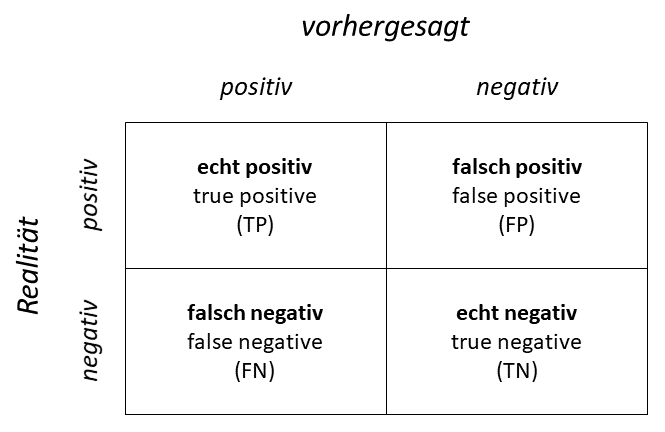
\includegraphics[width=0.7\textwidth]{images/Confusion}
    \caption{allgemeine Konfusionsmatrix\label{fig:confu}}
\end{figure}

Sowohl scitkit-learn als auch WEKA besitzen die Option, Konfisionsmatrizen zu den durchgeführten Tests der Klassifikatoren auszugeben. Anhand der Werte der Zuordnungen zu den zuvor genannten Gruppen wurden die folgenden Evaluationsmetriken berechnet: 

\begin{itemize}
\item Treffergenauigkeit (Accuracy)
\\Dieser Wert misst die Treffergenauigkeit der Vorhersagen des Klassifikators und gibt an, inwieweit dessen Vorhersagen mit der modellierten Realität übereinstimmen \cite{Sammut2017}. Die Formel zur Berechnung der Accuracy lautet:
\\\[Accuracy = \frac{TP+TN}{TP+TN+FP+FN}\]
Das Ergebnis der Berechnung ist ein prozentualer Wert. 100\% stellen damit die bestmögliche Accuracy dar.
\item Echt-Positiv-Rate / Trefferquote (TP-Rate / Recall)
\\Dieser Wert gibt den Anteil der korrekt als positiv gewerteten Vorhersagen sämtlicher als positiv gewerteter Vorhersagen an \cite{Alpaydin2010}. Die Formel zur Berechnung der TP-Rate bzw. des Recalls lautet:
\\\[TP-Rate = \frac{TP}{TP+FN}\]
Das Ergebnis der Berechnung ist ein prozentualer Wert. 100\% stellen damit die bestmögliche TP-Rate bzw. den bestmöglichen Recall dar. Beide Begriffe werden parallel für die Berechnung der gezeigten Formel verwendet.
\item Positiver Vorhersagewert (Precision)
\\ Dieser Wert gibt die Anzahl der positiven Vorhersagen an, die auch tatsächlich zur positiven Klasse gehören \cite{Sammut2017}. Die Formel zur Bestimmung der Precision lautet:
\\\[Precision = \frac{TP}{TP+FP}\]
Das Ergebnis der Berechnung ist ein prozentualer Wert. 100\% stellen damit die bestmögliche Precision dar.
\item F-Maß (F-Score)
\\ Dieser Wert berechnet das harmonische Mittel der Werte Precision und Recall und liegt somit zwischen diesen beiden Werten, jedoch näher am kleineren Wert \cite{Sammut2017}. Die Formel zur Berechnung des F-Scores lautet:
\\\[F-Score = \frac{2TP}{2TP+FP+FN}\]
Das Ergebnis der Berechnung ist ein prozentualer Wert. 100\% stellen damit den bestmöglichen F-Score dar.
\end{itemize}

Darüber hinaus wurden die sogenannten ROC-Kurven (ROC curve) der einzelnen Klassifikatoren ermittelt. Diese Wahrscheinlichkeitskurven bzw. -graphen (ROC = Receiver Operating characteristic, Betriebsverhalten des Empfängers), beschreiben das Verhältnis zwischen der TP-Rate (y-Achse) und der FP-Rate (x-Achse) \cite{Sammut2017,Narkhede2018}. Die Falsch-Positiv-Rate (FP-Rate) gibt dabei den Anteil der fälschlicherweise als positiv gewerteten Vorhersagen an \cite{Alpaydin2010}. Sie wird mittels der folgenden Formel berechnet:
\\\[FP-Rate = \frac{FP}{FP+TN}\]

Wie bei allen Metriken ist das Ergebnis der FP-Rate ein prozentualer Wert, der bestenfalls möglichst gering ausfallen sollte. Sowohl die TP-Rate als auch die FP-Rate geben nur singuläre Werte an, aus welchen sich keine Graphen herleiten lassen. Jeder Klassifikator errechnet jedoch im Rahmen der Vorhersage eines Datensatzes Wahrscheinlichkeiten, die die Zugehörigkeit zu den Werten der Zielklasse darstellen \cite{KNIMETV2019}. In der Regel wird ein Datenpunkt der positiven Klasse zugeordnet, wenn die Wahrscheinlichkeit einen Schwellenwert von 0,5 übersteigt - Datenpunkte, die diesen Schwellenwert unterschreiten werden wiederum der negativen Klasse zugeordnet \cite{KNIMETV2019}. Wird der Schwellenwert erhöht, so werden weniger Datenpunkte der positiven Klasse zugeordnet, wohingegen im Falle einer Absenkung des Schwellenwertes mehr Datenpunkte der positiven Klasse zugeordnet werden \cite{KNIMETV2019}. Für die Erstellung der ROC-Kurven werden somit die Werte der TP-Rate und der FP-Rate unter der Berücksichtigung der Schwellenwerte im Bereich von 0,0 bis 1,0 gegenübergestellt.

Eine weitere Metrik, die in Verbindung mit der ROC-Kurve auftritt, ist der ROC-Bereich (ROC area). Dieser Wert, der anhand der ROC-Kurve berechnet wird und auch AUC-Bereich (AUC = Area Under Curve, Bereich unter der Kurve) genannt wird, gibt an, in wieweit ein Klassifikator in der Lage ist, zwischen den Werten der Zielklassen zu unterscheiden \cite{Narkhede2018}. Je höher dieser Wert ist (1,0 ist das Maximum), desto besser trifft der Klassifikator korrekte Vorhersagen \cite{Narkhede2018}.

Am Beispiel des Schwellenwertes 0,5 wird nun die Interpretation der ROC-Kurve und des ROC-Bereiches vorgenommen. Unterstützt wird dies durch grafische Beispiele, die in \autoref{fig:curves} gezeigt werden. Der Idealfall ist in den (a) und (b) dargestellt. Die Wahrscheinlichkeitskurven der Zielklasse (a) weisen keine Überlappung auf. Die Werte der Zielklasse sind somit allesamt korrekt zugeordnet worden, sodass der Klassifikator korrekt zwischen diesen unterscheiden kann. Die diesem Fall entsprechende ROC-Kurve ist in (b) dargestellt. Der ROC-Bereich beträt in diesem Fall 1,0. Ein \glqq Normalfall\grqq{} ist in (c) und (d) dargestellt. Es ist in (c) zu erkennen, dass die Wahrscheinlichkeitskurven überlappen, sodass falsche Zuordnungen getroffen werden. Die entsprechende ROC-Kurve ist in (d) dargestellt. Der entsprechende ROC-Bereich beträgt im hier gezeigten Fall 0,7. Dies bedeutet, dass 70\% der Zuordnungen richtig getroffen werden. Verbessert werden können die Werte möglicherweise, wenn der Schwellenwert verändert wird. Der \glqq Worst Case\grqq, der bei der Performanzmessung mittels ROC-Kurven auftreten kann, ist in (e) und (f) dargestellt. In (e) ist zu erkennen, dass sich die Wahrscheinlichkeitskurven vollständig überlappen. Es findet somit eine willkürliche Zuordnung statt. Die zugehörige ROC-Kruve (f) entspricht einer Winkelhalbierenden. Ein weiterer Fehlerfall ist in (g) und (h) dargestellt. Die Wahrscheinlichkeitskurven (g) zeigen, dass die Zuordnungen gegenteilig erfolgen und somit der jeweils dem anderen Wert der Zielklasse falsch zugeordnet werden. Der entsprechende ROC-Bereich beträgt 0, da wie in (h) zu sehen ist, keine Fläche unter der Kurve vorhanden ist.

\begin{figure}
  \centering
  \subfloat[][Idealfall]{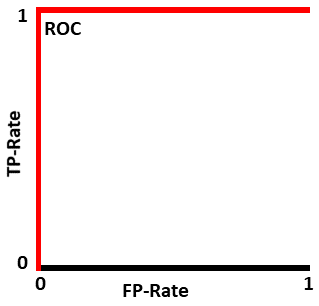
\includegraphics[width=0.5\linewidth]{images/roc_ideal}}
  \subfloat[][Idealfall]{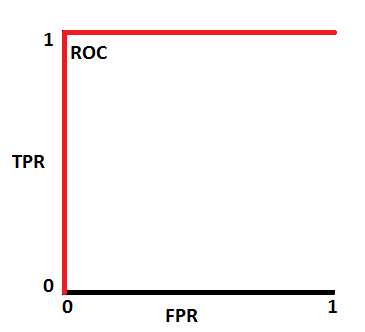
\includegraphics[width=0.25\linewidth]{images/roc_ideal_curve}}
  \qquad
  \subfloat[][\glqq Normalfall\grqq]{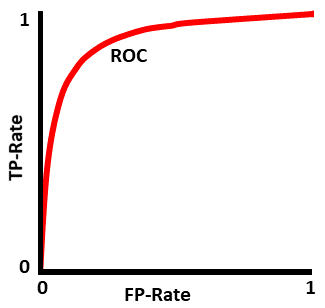
\includegraphics[width=0.5\linewidth]{images/roc_normal}}
  \subfloat[][\glqq Normalfall\grqq]{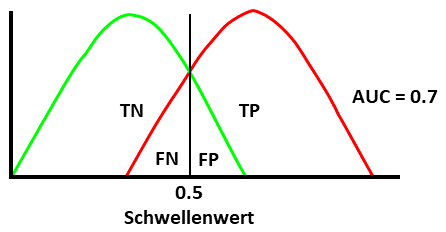
\includegraphics[width=0.25\linewidth]{images/roc_normal_curve}}
  \qquad
  \subfloat[][\glqq Worst Case\grqq]{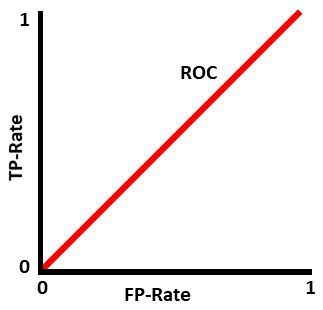
\includegraphics[width=0.5\linewidth]{images/roc_worst}}
  \subfloat[][\glqq Worst Case\grqq]{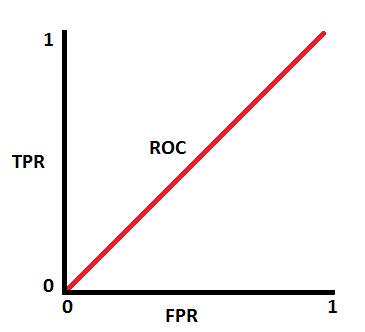
\includegraphics[width=0.25\linewidth]{images/roc_worst_curve}}
  \qquad
  \subfloat[][Fehlerfall]{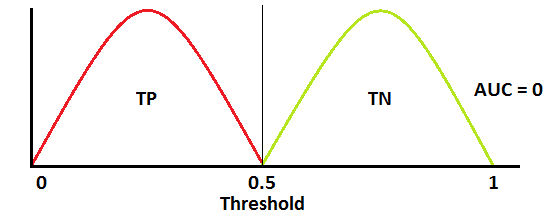
\includegraphics[width=0.5\linewidth]{images/roc_neg}}
  \subfloat[][Fehlerfall]{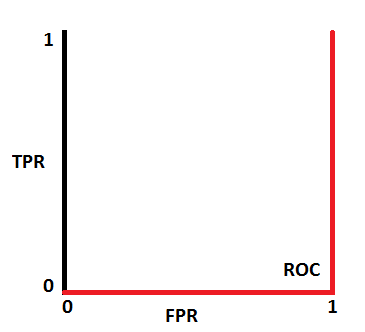
\includegraphics[width=0.25\linewidth]{images/roc_neg_curve}}
  \caption{Beispiel zur Interpretation der ROC-Kurve und des ROC-Bereiches (TPR = TP-Rate, FPR = FP-Rate, Threshold = Schwellenwert) \cite{Narkhede2018}
\label{fig:curves}}
\end{figure}

Alle vorgestellten Metriken werden automatisiert von den Werkzeugen scikit-learn und WEKA berechnet. Ferner besitzen beide Werkzeuge die Fähigkeit, ROC-Kurven mit den entsprechenden ROC-Werten auszugeben. Die im Rahmen der Evaluation der Klassifikatoren ermittelten Werte der Metriken sowie die ROC-Kurven und Werte der ROC-Bereiche werden im folgenden Abschnitt aufgeführt und gedeutet.

\fbox{\parbox{\linewidth}{RQ3a: WELCHE MITEINANDER VERGLEICHBAREN MERKMALE BESITZEN DIE KLASSIFIKATOREN?\medskip\\
Die Merkmale zum Vergleich stellen Evaluationsmetriken dar, welche anhand der Ergebnisse des Tests der Klassifikatoren errechnet werden und die Performanz der Vorhersagen auf verschiedene Weisen messen. Welche Metriken berechnet berechnet wurden beantwortet Forschungsfrage RQ3b.}}

\fbox{\parbox{\linewidth}{RQ3b: WELCHE METRIKEN KÖNNEN FÜR DEN VERGLEICH VERWENDET WERDEN?\medskip\\
Für den Vergleich der Klassifikatoren werden klassische Evaluationsmetriken verwendet, welche auf Basis der Konfusionsmatrizen berechnet werden. Ebenfalls hinzugezogen werden die jeweiligen ROC-Kurven der Klassifikatoren mit ihren ROC-Bereichen. Diese Metriken stellen einen Standard für die Messung von Klassifikatoren dar.}}

\subsection{Ergebnisse und Diskussion}
\label{results}

Dieser Abschnitt dient zur Präsentation der Ergebnisse der Evaluation der Klassifikatoren anhand der zuvor vorgestellten Evaluationsmetriken. Ferner werden die vorgestellten Ergebnisse innerhalb und zwischen der Datensets verglichen und interpretiert. 

\begin{table}[t]
\centering
\caption{Konfusionsmatrizen des featurebasierten Datensets}
\label{tab:mat-scikit}
\resizebox{\linewidth}{!}{%
\begin{tabular}{|>{\hspace{0pt}}p{0.073\linewidth}>{\hspace{0pt}}p{0.258\linewidth}|>{\RaggedLeft\hspace{0pt}}p{0.141\linewidth}>{\RaggedLeft\hspace{0pt}}p{0.098\linewidth}>{\RaggedLeft\hspace{0pt}}p{0.085\linewidth}|>{\RaggedLeft\hspace{0pt}}p{0.143\linewidth}>{\RaggedLeft\hspace{0pt}}p{0.1\linewidth}>{\RaggedLeft\hspace{0pt}}p{0.087\linewidth}|} 
\cline{3-8}
\multicolumn{1}{>{\hspace{0pt}}p{0.073\linewidth}}{}            &                                    & \multicolumn{3}{>{\Centering\hspace{0pt}}p{0.324\linewidth}|}{\textbf{scikit-learn} } & \multicolumn{3}{>{\Centering\hspace{0pt}}p{0.329\linewidth}|}{\textbf{WEKA} }  \\ 
\cline{2-8}
\multicolumn{1}{>{\Centering\hspace{0pt}}p{0.073\linewidth}|}{} & \textbf{Ermittelt -\textgreater{}} & \textbf{Fehlerfrei}  & \textbf{Defekt}  & \textbf{Total}                              & \textbf{Fehlerfrei}  & \textbf{Defekt}  & \textbf{Total}                       \\ 
\hline
\multirow{3}{0.073\linewidth}{\hspace{0pt}DT}                   & Realität fehlerfrei                & 1.627                & 122              & 1.749                                       & 3.285                & 188              & 3.473                                \\
                                                                & Realität defekt                    & 146                  & 268              & 414                                         & 388                  & 463              & 851                                  \\
                                                                & Total                              & 1.773                & 390              & 2.163                                       & 3.673                & 651              & 4.324                                \\ 
\hline
\multirow{3}{0.073\linewidth}{\hspace{0pt}KNN}                  & Realität fehlerfrei                & 2.691                & 241              & 2.932                                       & 3.781                & 276              & 4.057                                \\
                                                                & Realität defekt                    & 255                  & 417              & 672                                         & 392                  & 596              & 988                                  \\
                                                                & Total                              & 2.946                & 658              & 3.604                                       & 4.173                & 875              & 5.045                                \\ 
\hline
\multirow{3}{0.073\linewidth}{\hspace{0pt}LR}                   & Realität fehlerfrei~ ~~            &                      &                  &                                             & 3.993                & 64               & 4.057                                \\
                                                                & Realität defekt                    &                      &                  &                                             & 737                  & 251              & 988                                  \\
                                                                & Total                              &                      &                  &                                             & 4.730                & 315              & 5.045                                \\ 
\hline
\multirow{3}{0.073\linewidth}{\hspace{0pt}NB}                   & Realität fehlerfrei                & 2.301                & 608              & 2.909                                       & 3.411                & 62               & 3.473                                \\
                                                                & Realität defekt                    & 648                  & 47               & 695                                         & 643                  & 208              & 851                                  \\
                                                                & Total                              & 2.949                & 655              & 3.604                                       & 4.054                & 270              & 4.324                                \\ 
\hline
\multirow{3}{0.073\linewidth}{\hspace{0pt}NN}                   & Realität fehlerfrei                & 1.692                & 99               & 1.791                                       & 2.175                & 120              & 2.395                                \\
                                                                & Realität defekt                    & 159                  & 213              & 372                                         & 315                  & 273              & 588                                  \\
                                                                & Total                              & 1.851                & 312              & 2.163                                       & 2.490                & 393              & 2.883                                \\ 
\hline
\multirow{3}{0.073\linewidth}{\hspace{0pt}RC}                   & Realität fehlerfrei                & 2.926                & 8                & 2.934                                       &                      &                  &                                      \\
                                                                & Realität defekt                    & 603                  & 67               & 670                                         &                      &                  &                                      \\
                                                                & Total                              & 3.529                & 75               & 3.604                                       &                      &                  &                                      \\ 
\hline
\multirow{3}{0.073\linewidth}{\hspace{0pt}RF}                   & Realität fehlerfrei                & 2.851                & 99               & 2.950                                       & 2.234                & 61               & 2.295                                \\
                                                                & Realität defekt                    & 213                  & 441              & 654                                         & 195                  & 393              & 588                                  \\
                                                                & Total                              & 3.064                & 540              & 3.604                                       & 2.429                & 454              & 2.883                                \\ 
\hline
\multirow{3}{0.073\linewidth}{\hspace{0pt}SGD}                  & Realität fehlerfrei                & 3.336                & 191              & 3.527                                       & 3.453                & 20               & 3.473                                \\
                                                                & Realität defekt                    & 613                  & 185              & 798                                         & 720                  & 131              & 851                                  \\
                                                                & Total                              & 3.949                & 376              & 4.325                                       & 4.173                & 151              & 4.324                                \\ 
\hline
\multirow{3}{0.073\linewidth}{\hspace{0pt}SVM}                  & Realität fehlerfrei                & 4.039                & 58               & 4.097                                       & 4.055                & 2                & 4.057                                \\
                                                                & Realität defekt                    & 722                  & 226              & 948                                         & 945                  & 43               & 988                                  \\
                                                                & Total                              & 4.761                & 284              & 5.045                                            & 5.000                & 45               & 5.045                                \\
\hline
\end{tabular}
}
\end{table}


\begin{table}[t]
\centering
\caption{Konfusionsmatrizen des dateibasierten Datensets}
\label{tab:mat-weka}
\resizebox{\linewidth}{!}{%
\begin{tabular}{|>{\hspace{0pt}}p{0.073\linewidth}>{\hspace{0pt}}p{0.241\linewidth}|>{\RaggedLeft\hspace{0pt}}p{0.139\linewidth}>{\RaggedLeft\hspace{0pt}}p{0.096\linewidth}>{\RaggedLeft\hspace{0pt}}p{0.098\linewidth}|>{\RaggedLeft\hspace{0pt}}p{0.139\linewidth}>{\RaggedLeft\hspace{0pt}}p{0.098\linewidth}>{\RaggedLeft\hspace{0pt}}p{0.1\linewidth}|} 
\cline{3-8}
\multicolumn{1}{>{\hspace{0pt}}p{0.073\linewidth}}{}            &                                      & \multicolumn{3}{>{\Centering\hspace{0pt}}p{0.333\linewidth}|}{\textbf{scikit-learn} }                                                                                                                                                                & \multicolumn{3}{>{\Centering\hspace{0pt}}p{0.337\linewidth}|}{\textbf{WEKA} }                                                                                                                                                                       \\ 
\cline{2-8}
\multicolumn{1}{>{\Centering\hspace{0pt}}p{0.073\linewidth}|}{} & \textbf{Ermittelt -\textgreater{}}   & \multicolumn{1}{>{\Centering\hspace{0pt}}p{0.139\linewidth}}{\textbf{Fehlerfrei} } & \multicolumn{1}{>{\Centering\hspace{0pt}}p{0.096\linewidth}}{\textbf{Defekt} } & \multicolumn{1}{>{\Centering\hspace{0pt}}p{0.098\linewidth}|}{\textbf{Total} } & \multicolumn{1}{>{\Centering\hspace{0pt}}p{0.139\linewidth}}{\textbf{Fehlerfrei} } & \multicolumn{1}{>{\Centering\hspace{0pt}}p{0.098\linewidth}}{\textbf{Defekt} } & \multicolumn{1}{>{\Centering\hspace{0pt}}p{0.1\linewidth}|}{\textbf{Total} }  \\ 
\hline
\multirow{3}{0.073\linewidth}{\hspace{0pt}J48}                  & Realität fehlerfrei                  & 21.704                                                                             & 121                                                                            & 21.825                                                                         & 21.320                                                                             & 464                                                                            & 21.784                                                                        \\
                                                                & Realität defekt                      & 1.905                                                                              & 12.782                                                                         & 14.687                                                                         & 693                                                                                & 14.034                                                                         & 14.727                                                                        \\
                                                                & Total                                & 23.609                                                                             & 12.903                                                                         & 36.512                                                                         & 22.013                                                                             & 14.498                                                                         & 36.511                                                                        \\ 
\hline
\multirow{3}{0.073\linewidth}{\hspace{0pt}KNN}                  & Realität fehlerfrei                  & 15.519                                                                             & 1.853                                                                          & 17.372                                                                         & 12.090                                                                             & 1.026                                                                          & 13.116                                                                        \\
                                                                & Realität defekt                      & 1.026                                                                              & 10.812                                                                         & 11.838                                                                         & 1.137                                                                              & 7.654                                                                          & 8.791                                                                         \\
                                                                & Total                                & 16.545                                                                             & 12.665                                                                         & 29.210                                                                         & 13.227                                                                             & 8.680                                                                          & 21.907                                                                        \\ 
\hline
\multirow{3}{0.073\linewidth}{\hspace{0pt}LR}                   & Realität fehlerfrei                  &                                                                                    &                                                                                &                                                                                & 28.023                                                                             & 2.570                                                                          & 30.593                                                                        \\
                                                                & Realität defekt                      &                                                                                    &                                                                                &                                                                                & 15.542                                                                             & 4.981                                                                          & 20.523                                                                        \\
                                                                & Total                                &                                                                                    &                                                                                &                                                                                & 43.565                                                                             & 7.551                                                                          & 51.116                                                                        \\ 
\hline
\multirow{3}{0.073\linewidth}{\hspace{0pt}NB}                   & Realität fehlerfrei                  & 8.667                                                                              & 4.368                                                                          & 13.035                                                                         & 18.982                                                                             & 2.802                                                                          & 21.784                                                                        \\
                                                                & Realität defekt                      & 3.212                                                                              & 5.660                                                                          & 8.872                                                                          & 10.369                                                                             & 4.358                                                                          & 14.727                                                                        \\
                                                                & Total                                & 11.879                                                                             & 10.028                                                                         & 21.907                                                                         & 29.351                                                                             & 7.160                                                                          & 36.511                                                                        \\ 
\hline
\multirow{3}{0.073\linewidth}{\hspace{0pt}NN}                   & Realität fehlerfrei                  & 20.904                                                                             & 744                                                                            & 21.648                                                                         & 18.754                                                                             & 3.030                                                                          & 21.784                                                                        \\
                                                                & Realität defekt                      & 3.522                                                                              & 11.342                                                                         & 14.864                                                                         & 8.619                                                                              & 6.108                                                                          & 14.727                                                                        \\
                                                                & Total                                & 24.426                                                                             & 12.086                                                                         & 36.512                                                                         & 27.373                                                                             & 9.138                                                                          & 36.511                                                                        \\ 
\hline
\multirow{3}{0.073\linewidth}{\hspace{0pt}RC}                   & Realität fehlerfrei\textasciitilde{} & 15.874                                                                             & 1.438                                                                          & 17.312                                                                         &                                                                                    &                                                                                &                                                                               \\
                                                                & Realität defekt                      & 9.152                                                                              & 2.746                                                                          & 11.898                                                                         &                                                                                    &                                                                                &                                                                               \\
                                                                & Total                                & 25.026                                                                             & 4.184                                                                          & 29.210                                                                         &                                                                                    &                                                                                &                                                                               \\ 
\hline
\multirow{3}{0.073\linewidth}{\hspace{0pt}RF}                   & Realität fehlerfrei                  & 17.189                                                                             & 212                                                                            & 17.401                                                                         & 12.990                                                                             & 126                                                                            & 13.116                                                                        \\
                                                                & Realität defekt                      & 374                                                                                & 11.435                                                                         & 11.809                                                                         & 275                                                                                & 8.516                                                                          & 8.791                                                                         \\
                                                                & Total                                & 17.563                                                                             & 11.647                                                                         & 29.210                                                                         & 13.265                                                                             & 8.642                                                                          & 21.907                                                                        \\ 
\hline
\multirow{3}{0.073\linewidth}{\hspace{0pt}SGD}                  & Realität fehlerfrei                  & 20.600                                                                             & 10.037                                                                         & 30.637                                                                         & 12.698                                                                             & 418                                                                            & 13.116                                                                        \\
                                                                & Realität defekt                      & 11.187                                                                             & 9.293                                                                          & 20.480                                                                         & 7.760                                                                              & 1.031                                                                          & 8.791                                                                         \\
                                                                & Total                                & 31.787                                                                             & 19.330                                                                         & 51.117                                                                         & 20.458                                                                             & 1.449                                                                          & 21.907                                                                        \\ 
\hline
\multirow{3}{0.073\linewidth}{\hspace{0pt}SVM}                  & Realität fehlerfrei                  & 28.190                                                                             & 2.237                                                                          & 30.427                                                                         & 12.679                                                                             & 437                                                                            & 13.116                                                                        \\
                                                                & Realität defekt                      & 16.479                                                                             & 4.211                                                                          & 20.690                                                                         & 7.816                                                                              & 975                                                                            & 8.791                                                                         \\
                                                                & Total                                & 44.669                                                                             & 6.448                                                                          & 51.117                                                                         & 20.495                                                                             & 1.412                                                                          & 21.907                                                                        \\
\hline
\end{tabular}
}
\end{table}

\begin{figure}
  \centering
  \subfloat[][DT (scikit)]{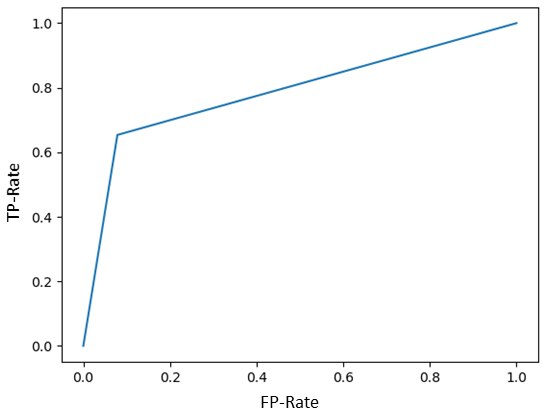
\includegraphics[width=0.25\linewidth]{images/dt_scikit}}
  \subfloat[][J48 (WEKA)]{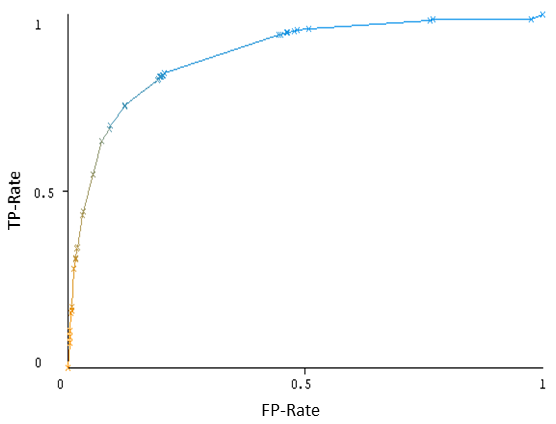
\includegraphics[width=0.25\linewidth]{images/j48_weka}}
  \subfloat[][NN (scikit)]{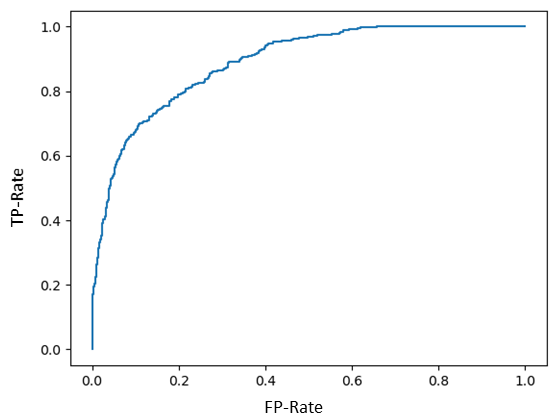
\includegraphics[width=0.25\linewidth]{images/nn_scikit}}
  \subfloat[][NN (WEKA)]{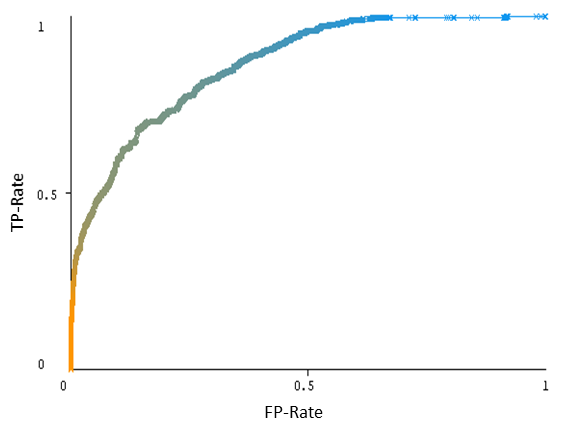
\includegraphics[width=0.25\linewidth]{images/nn_weka}}
  \qquad
  \subfloat[][KNN (scikit)]{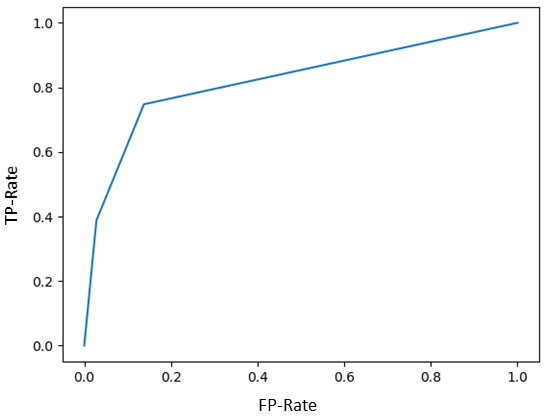
\includegraphics[width=0.25\linewidth]{images/knn_scikit}}
  \subfloat[][KNN (WEKA)]{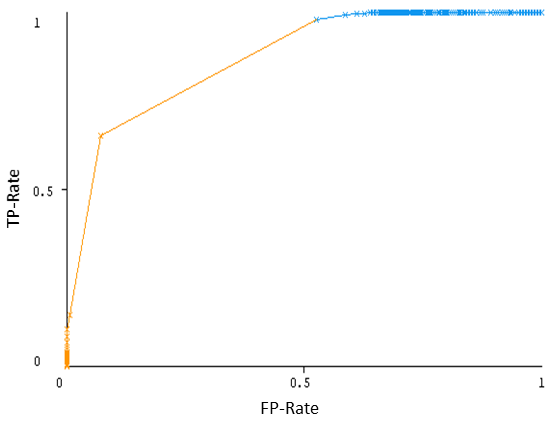
\includegraphics[width=0.25\linewidth]{images/knn_weka}}
  \subfloat[][RF (scikit)]{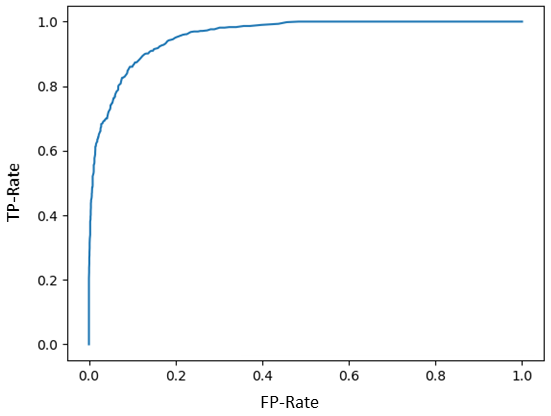
\includegraphics[width=0.25\linewidth]{images/rf_scikit}}
  \subfloat[][RF (WEKA)]{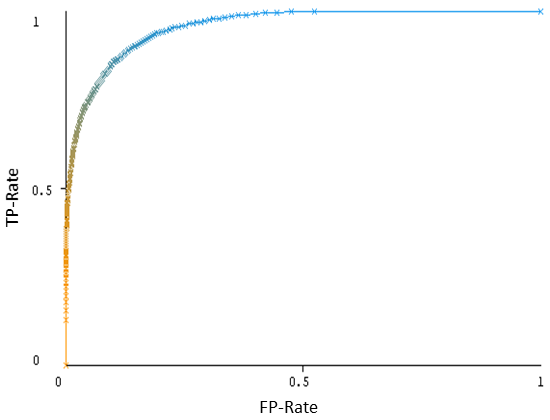
\includegraphics[width=0.25\linewidth]{images/rf_weka}}
  \qquad
  \subfloat[][RC (scikit)]{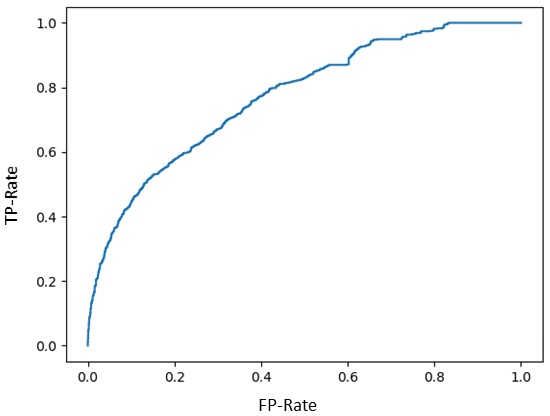
\includegraphics[width=0.25\linewidth]{images/rc_scikit}}
  \subfloat[][LR (WEKA)]{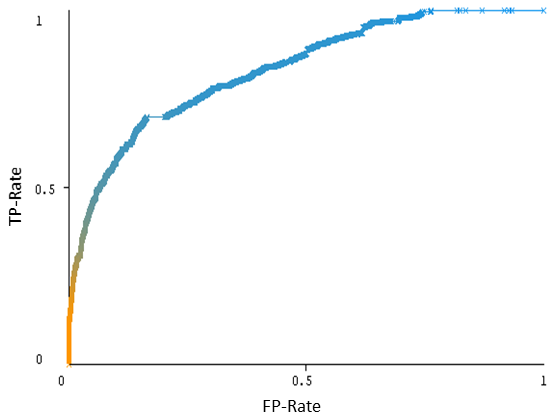
\includegraphics[width=0.25\linewidth]{images/lr_weka}}
  \subfloat[][SGD (scikit)]{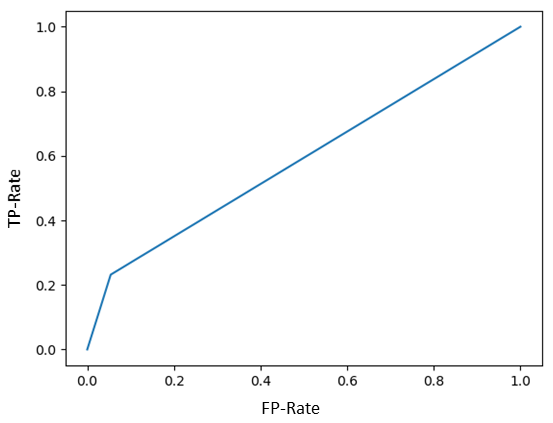
\includegraphics[width=0.25\linewidth]{images/sgd_scikit}}
  \subfloat[][SGD (WEKA)]{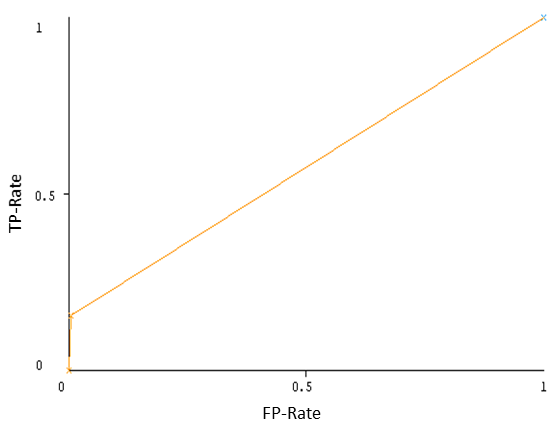
\includegraphics[width=0.25\linewidth]{images/sgd_weka}}
  \qquad
  \subfloat[][NB (scikit)]{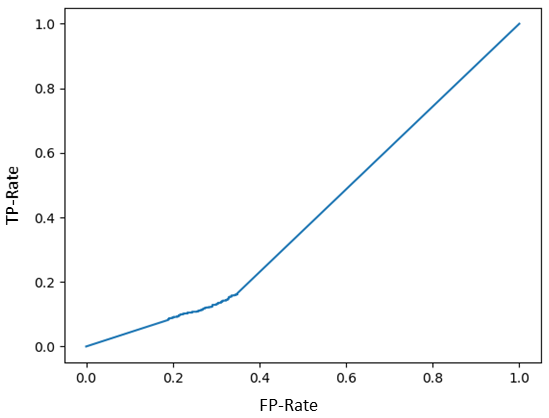
\includegraphics[width=0.25\linewidth]{images/nb_scikit}}
  \subfloat[][NB (WEKA)]{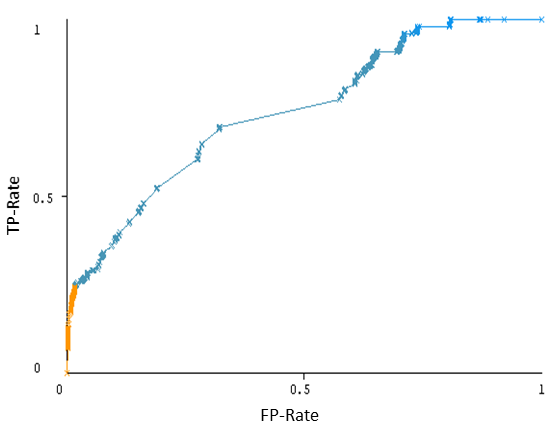
\includegraphics[width=0.25\linewidth]{images/nb_weka}}
  \subfloat[][SVM (scikit)]{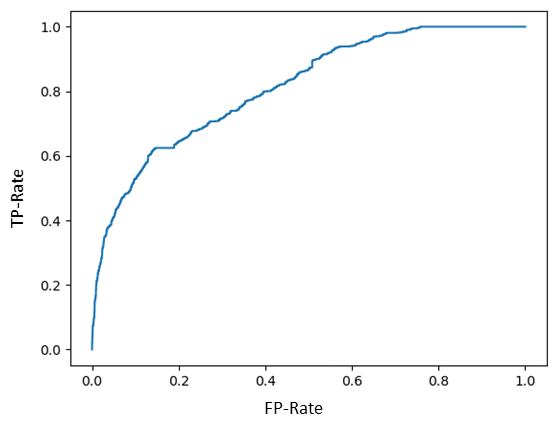
\includegraphics[width=0.25\linewidth]{images/svm_scikit}}
  \subfloat[][SVM (WEKA)]{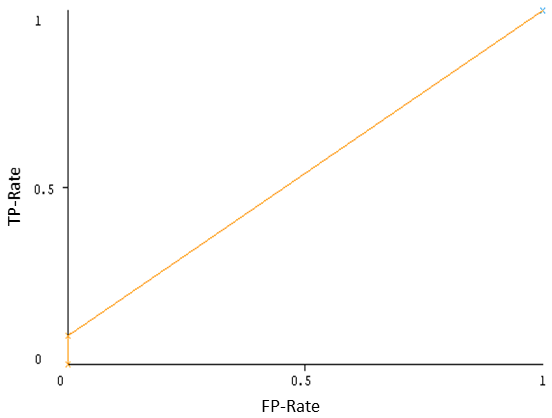
\includegraphics[width=0.25\linewidth]{images/svm_weka}}
  \caption{ROC-Kurven der Klassifikatoren des featurebasierten Datensets}
\end{figure}

\begin{figure}
  \centering
  \subfloat[][DT (scikit)]{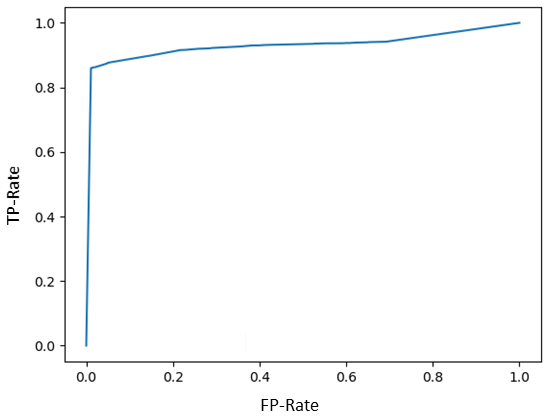
\includegraphics[width=0.25\linewidth]{images/dt_scikit_file}}
  \subfloat[][J48 (WEKA)]{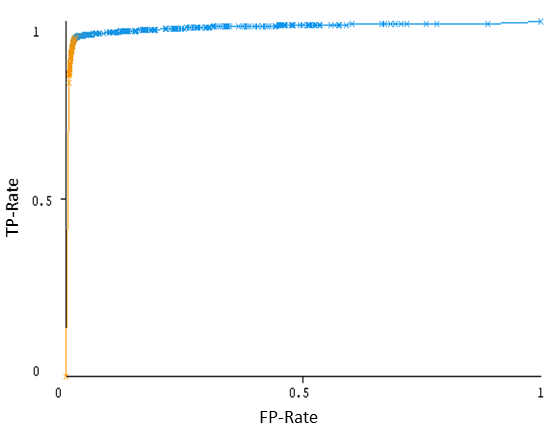
\includegraphics[width=0.25\linewidth]{images/j48_weka_file}}
  \subfloat[][NN (scikit)]{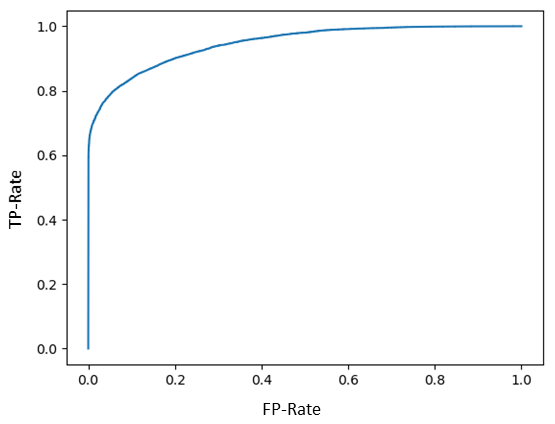
\includegraphics[width=0.25\linewidth]{images/nn_scikit_file}}
  \subfloat[][NN (WEKA)]{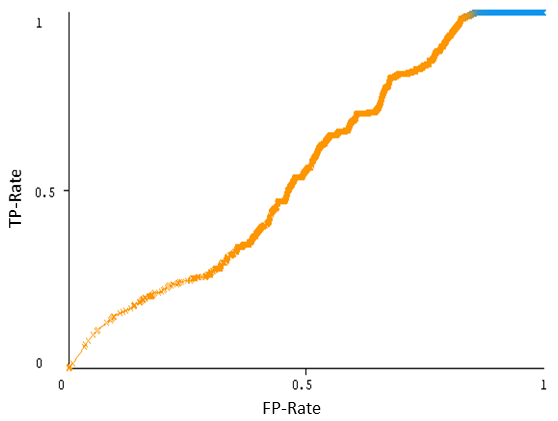
\includegraphics[width=0.25\linewidth]{images/nn_weka_file}}
  \qquad
  \subfloat[][KNN (scikit)]{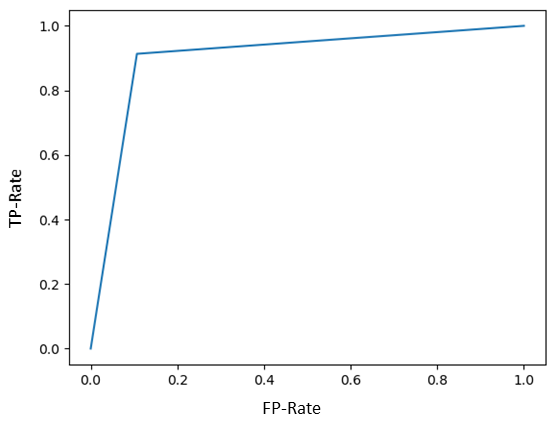
\includegraphics[width=0.25\linewidth]{images/knn_scikit_file}}
  \subfloat[][KNN (WEKA)]{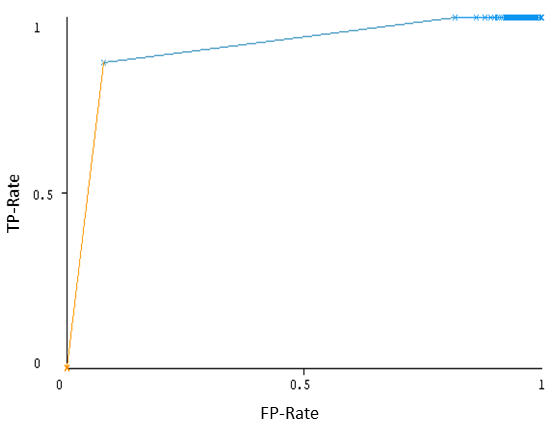
\includegraphics[width=0.25\linewidth]{images/knn_weka_file}}
  \subfloat[][RF (scikit)]{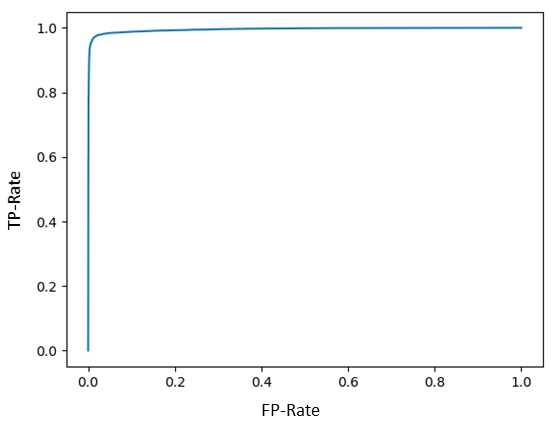
\includegraphics[width=0.25\linewidth]{images/rf_scikit_file}}
  \subfloat[][RF (WEKA)]{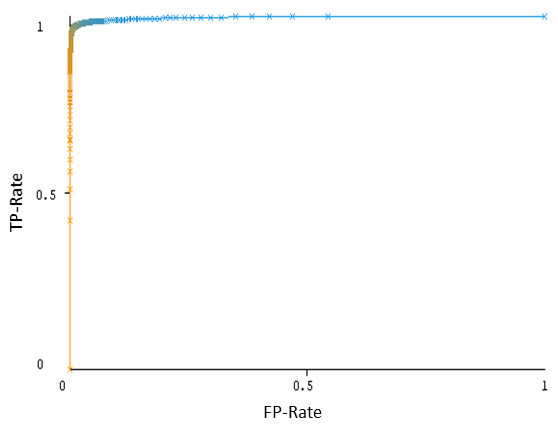
\includegraphics[width=0.25\linewidth]{images/rf_weka_file}}
  \qquad
  \subfloat[][RC (scikit)]{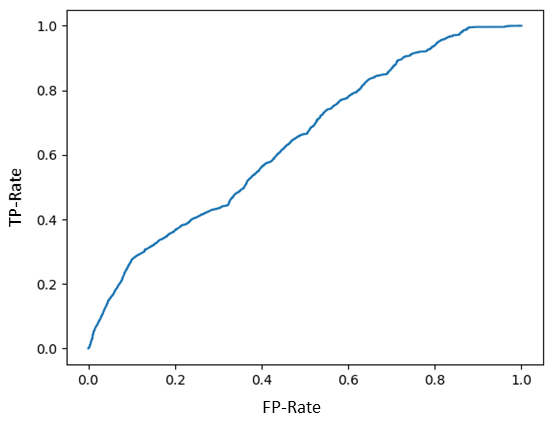
\includegraphics[width=0.25\linewidth]{images/rc_scikit_file}}
  \subfloat[][LR (WEKA)]{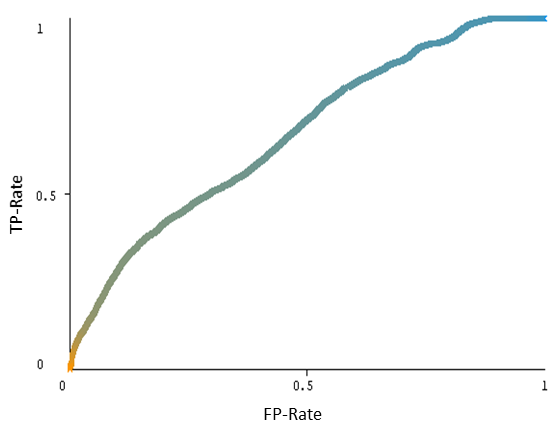
\includegraphics[width=0.25\linewidth]{images/lr_weka_file}}
  \subfloat[][SGD (scikit)]{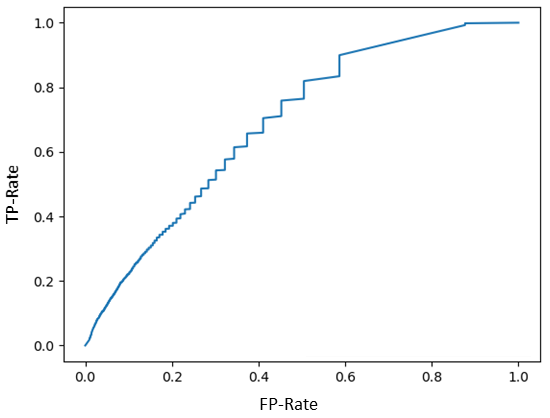
\includegraphics[width=0.25\linewidth]{images/sgd_scikit_file}}
  \subfloat[][SGD (WEKA)]{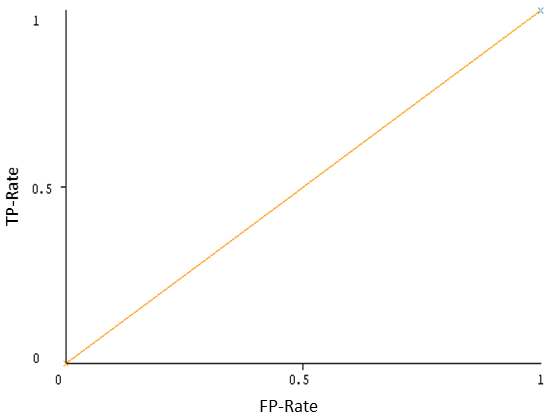
\includegraphics[width=0.25\linewidth]{images/sgd_weka_file}}
  \qquad
  \subfloat[][NB (scikit)]{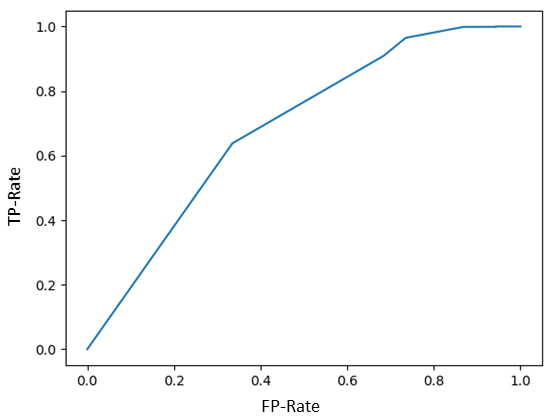
\includegraphics[width=0.25\linewidth]{images/nb_scikit_file}}
  \subfloat[][NB (WEKA)]{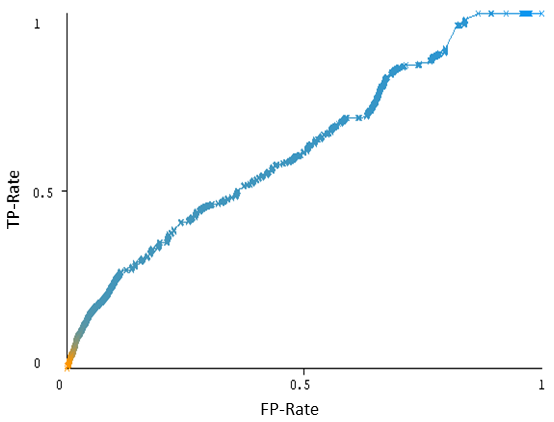
\includegraphics[width=0.25\linewidth]{images/nb_weka_file}}
  \subfloat[][SVM (scikit)]{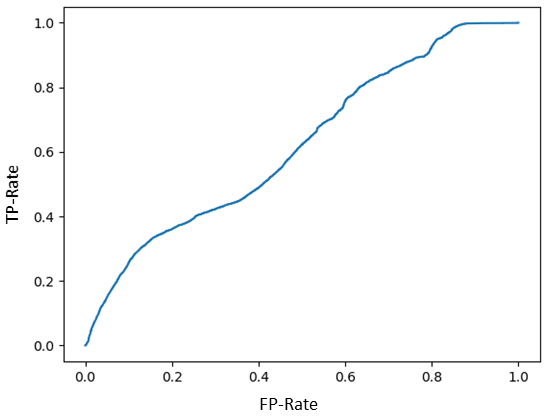
\includegraphics[width=0.25\linewidth]{images/svm_scikit_file}}
  \subfloat[][SVM (WEKA)]{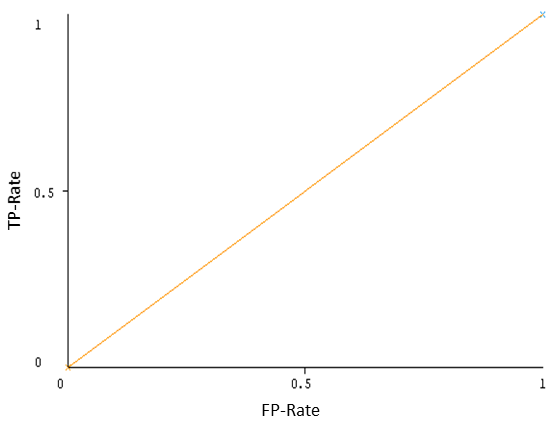
\includegraphics[width=0.25\linewidth]{images/svm_weka_file}}
  \caption{ROC-Kurven der Klassifikatoren des dateibasierten Datensets}
\end{figure}

\begin{figure}
  \centering
  \subfloat[][scikit]{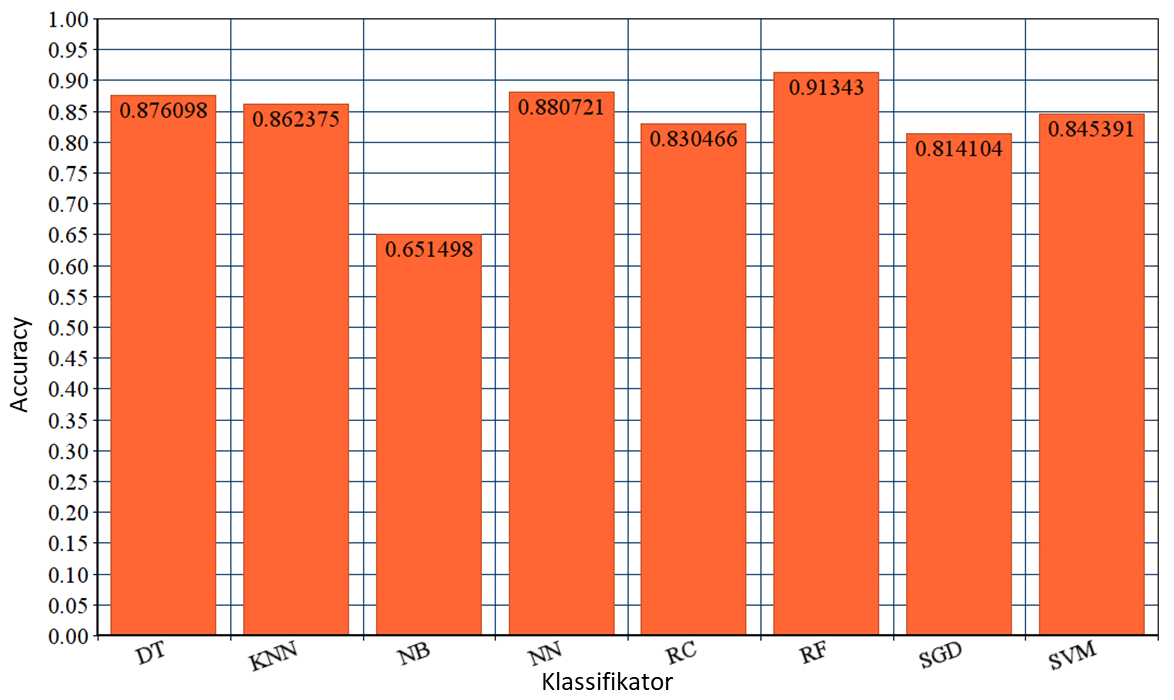
\includegraphics[width=0.5\linewidth]{images/feat_final_scikit}}
  \subfloat[][WEKA]{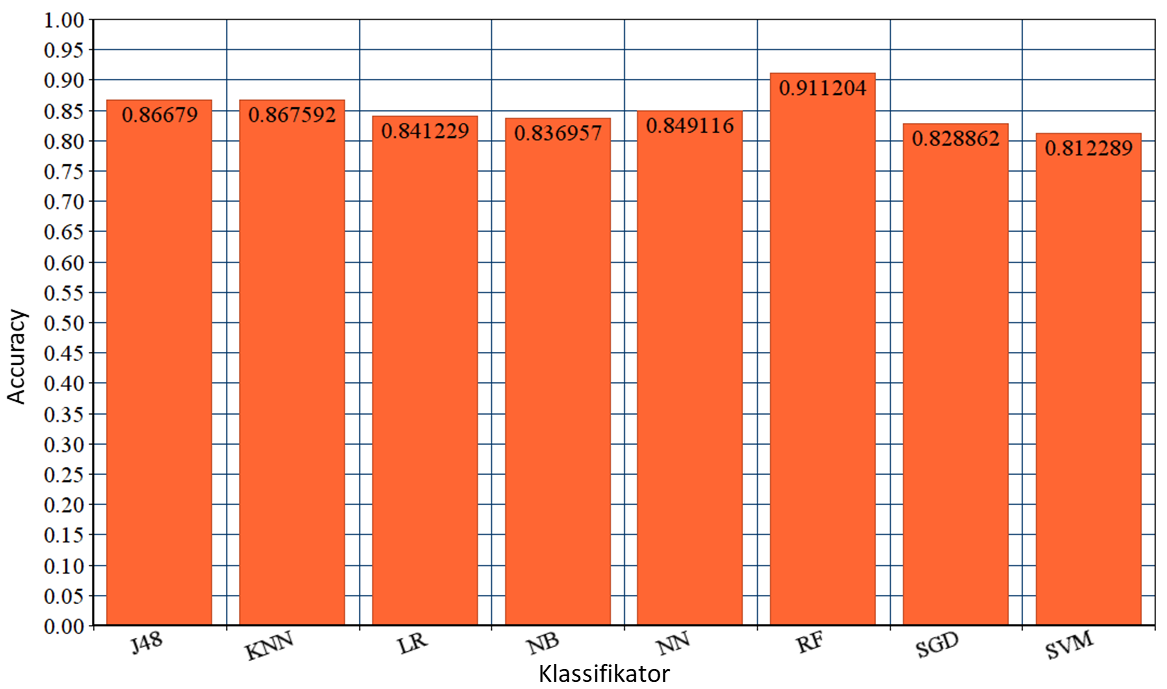
\includegraphics[width=0.5\linewidth]{images/feat_final_weka}}
  \caption{Vergleich der Accuracies der featurebasierten Klassifikatoren von scikit-learn und WEKA\label{fig:final-feat}}
\end{figure}

\begin{figure}
  \centering
  \subfloat[][scikit]{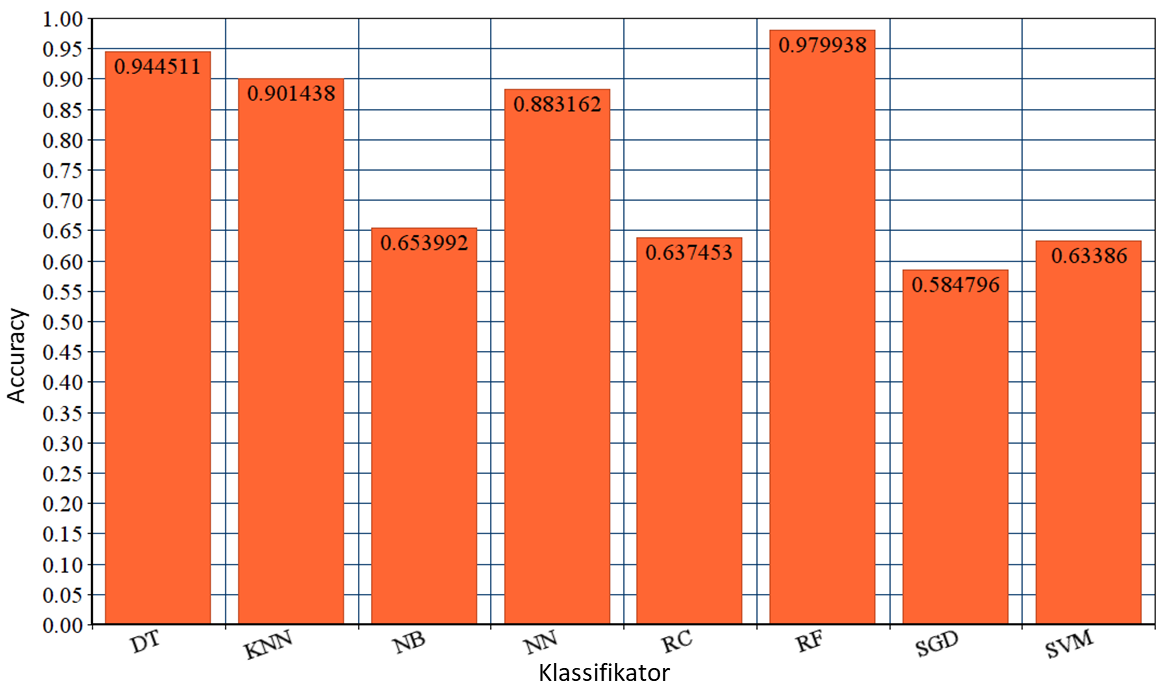
\includegraphics[width=0.5\linewidth]{images/file_final_scikit}}
  \subfloat[][WEKA]{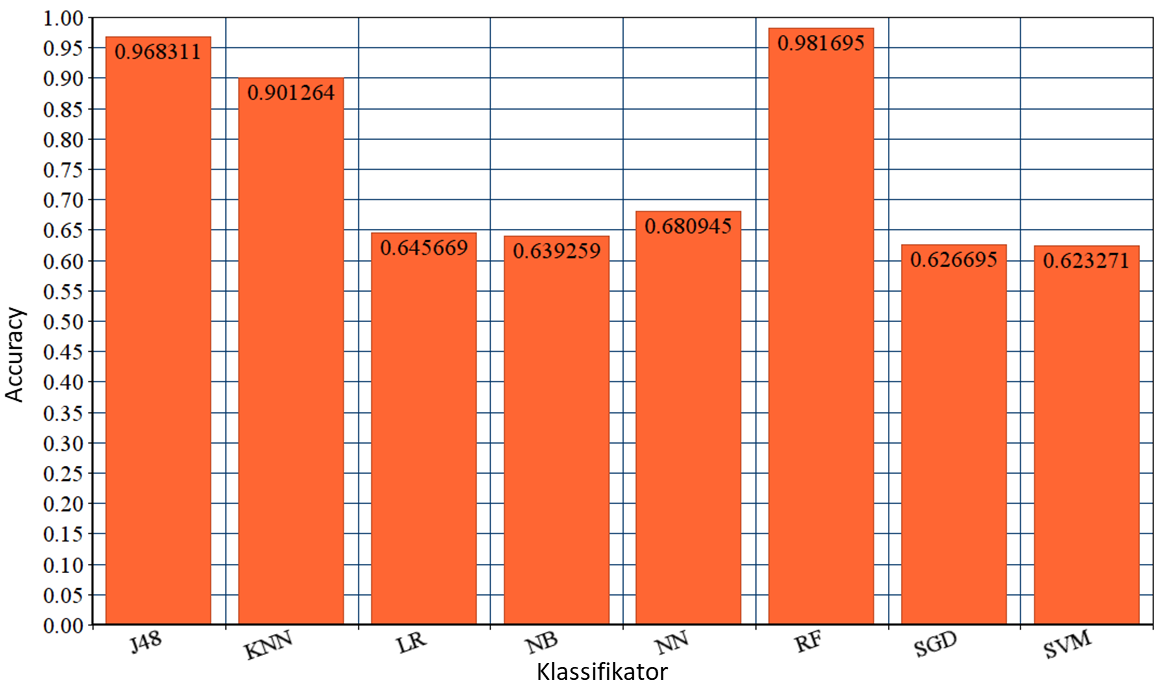
\includegraphics[width=0.5\linewidth]{images/file_final_weka}}
  \caption{Vergleich der Accuracies der dateibasierten Klassifikatoren von scikit-learn und WEKA\label{fig:final-file}}
\end{figure}

\begin{table}[t]
\centering
\caption{Ergebnisse der Evaluationsmetriken des featurebasierten Datensets}
\label{tab:met-scikit}
\resizebox{\linewidth}{!}{%
\begin{tabular}{|>{\hspace{0pt}}p{0.081\linewidth}>{\hspace{0pt}}p{0.16\linewidth}|>{\RaggedLeft\hspace{0pt}}p{0.156\linewidth}>{\RaggedLeft\hspace{0pt}}p{0.11\linewidth}>{\RaggedLeft\hspace{0pt}}p{0.097\linewidth}|>{\RaggedLeft\hspace{0pt}}p{0.156\linewidth}>{\RaggedLeft\hspace{0pt}}p{0.11\linewidth}>{\RaggedLeft\hspace{0pt}}p{0.098\linewidth}|} 
\cline{3-8}
\multicolumn{1}{>{\hspace{0pt}}p{0.081\linewidth}}{}           &           & \multicolumn{3}{>{\Centering\hspace{0pt}}p{0.363\linewidth}|}{\textbf{scikit-learn}} & \multicolumn{3}{>{\Centering\hspace{0pt}}p{0.364\linewidth}|}{\textbf{WEKA}}   \\ 
\cline{3-8}
\multicolumn{1}{>{\Centering\hspace{0pt}}p{0.081\linewidth}}{} &           & \textbf{Fehlerfrei}  & \textbf{Defekt}  & \textbf{gew.}\par{}\textbf{Mittel}         & \textbf{Fehlerfrei}  & \textbf{Defekt}  & \textbf{gew.}\par{}\textbf{Mittel}   \\ 
\hline
\multirow{4}{0.081\linewidth}{\hspace{0pt}DT}                  & Precision & 0,92                 & 0,69             & 0,87                                       & 0,89                 & 0,71             & 0,86                                 \\
                                                               & Recall    & 0,93                 & 0,65             & 0,88                                       & 0,95                 & 0,54             & 0,87                                 \\
                                                               & F-Score   & 0,92                 & 0,67             & 0,87                                       & 0,92                 & 0,62             & 0,86                                 \\
                                                               & ROC-Area  & 0,79                 & 0,79             & 0,79                                       & 0,88                 & 0,88             & 0,88                                 \\ 
\hline
\multirow{4}{0.081\linewidth}{\hspace{0pt}KNN}                 & Precision & 0,91                 & 0,63             & 0,86                                       & 0,91                 & 0,63             & 0,86                                 \\
                                                               & Recall    & 0,92                 & 0,62             & 0,86                                       & 0,93                 & 0,60             & 0,87                                 \\
                                                               & F-Score   & 0,92                 & 0,63             & 0,86                                       & 0,92                 & 0,64             & 0,86                                 \\
                                                               & ROC-Area  & 0,77                 & 0,77             & 0,77                                       & 0,85                 & 0,85             & 0,85                                 \\ 
\hline
\multirow{4}{0.081\linewidth}{\hspace{0pt}LR}                  & Precision &                      &                  &                                            & 0,84                 & 0,80             & 0,83                                 \\
                                                               & Recall    &                      &                  &                                            & 0,99                 & 0,25             & 0,84                                 \\
                                                               & F-Score   &                      &                  &                                            & 0,91                 & 0,39             & 0,81                                 \\
                                                               & ROC-Area  &                      &                  &                                            & 0,82                 & 0,82             & 0,82                                 \\ 
\hline
\multirow{4}{0.081\linewidth}{\hspace{0pt}NB}                  & Precision & 0,78                 & 0,07             & 0,64                                       & 0,81                 & 0,77             & 0,83                                 \\
                                                               & Recall    & 0,79                 & 0,07             & 0,65                                       & 0,98                 & 0,24             & 0,84                                 \\
                                                               & F-Score   & 0,79                 & 0,07             & 0,65                                       & 0,91                 & 0,37             & 0,80                                 \\
                                                               & ROC-Area  & 0,41                 & 0,41             & 0,41                                       & 0,74                 & 0,74             & 0,74                                 \\ 
\hline
\multirow{4}{0.081\linewidth}{\hspace{0pt}NN}                  & Precision & 0,91                 & 0,68             & 0,87                                       & 0,87                 & 0,70             & 0,84                                 \\
                                                               & Recall    & 0,94                 & 0,57             & 0,88                                       & 0,95                 & 0,46             & 0,85                                 \\
                                                               & F-Score   & 0,93                 & 0,92             & 0,88                                       & 0,91                 & 0,56             & 0,84                                 \\
                                                               & ROC-Area  & 0,89                 & 0,89             & 0,89                                       & 0,86                 & 0,86             & 0,86                                 \\ 
\hline
\multirow{4}{0.081\linewidth}{\hspace{0pt}RC}                  & Precision & 0,83                 & 0,89             & 0,84                                       &                      &                  &                                      \\
                                                               & Recall    & 1,00                 & 0,10             & 0,83                                       &                      &                  &                                      \\
                                                               & F-Score   & 0,91                 & 0,18             & 0,77                                       &                      &                  &                                      \\
                                                               & ROC-Area  & 0,77                 & 0,77             & 0,77                                       &                      &                  &                                      \\ 
\hline
\multirow{4}{0.081\linewidth}{\hspace{0pt}RF}                  & Precision & 0,93                 & 0,82             & 0,91                                       & 0,92                 & 0,87             & 0,91                                 \\
                                                               & Recall    & 0,97                 & 0,67             & 0,91                                       & 0,97                 & 0,67             & 0,91                                 \\
                                                               & F-Score   & 0,95                 & 0,74             & 0,91                                       & 0,95                 & 0,75             & 0,91                                 \\
                                                               & ROC-Area  & 0,95                 & 0,95             & 0,95                                       & 0,95                 & 0,95             & 0,95                                 \\ 
\hline
\multirow{4}{0.081\linewidth}{\hspace{0pt}SGD}                 & Precision & 0,84                 & 0,49             & 0,78                                       & 0,83                 & 0,87             & 0,84                                 \\
                                                               & Recall    & 0,95                 & 0,23             & 0,81                                       & 0,99                 & 0,15             & 0,83                                 \\
                                                               & F-Score   & 0,89                 & 0,32             & 0,81                                       & 0,90                 & 0,26             & 0,78                                 \\
                                                               & ROC-Area  & 0,59                 & 0,59             & 0,59                                       & 0,57                 & 0,57             & 0,57                                 \\ 
\hline
\multirow{4}{0.081\linewidth}{\hspace{0pt}SVM}                 & Precision & 0,85                 & 0,80             & 0,84                                       & 0,81                 & 0,96             & 0,84                                 \\
                                                               & Recall    & 0,99                 & 0,24             & 0,85                                       & 1,00                 & 0,04             & 0,81                                 \\
                                                               & F-Score   & 0,91                 & 0,37             & 0,81                                       & 0,90                 & 0,08             & 0,74                                 \\
                                                               & ROC-Area  & 0,81                 & 0,81             & 0,81                                       & 0,52                 & 0,52             & 0,52                                 \\
\hline
\end{tabular}
}
\end{table}

\begin{table}[t]
\centering
\caption{Ergebnisse der Evaluationsmetriken des dateibasierten Datensets}
\label{tab:met-file}
\resizebox{\linewidth}{!}{%
\begin{tabular}{|>{\hspace{0pt}}p{0.085\linewidth}>{\hspace{0pt}}p{0.164\linewidth}|>{\RaggedLeft\hspace{0pt}}p{0.151\linewidth}>{\RaggedLeft\hspace{0pt}}p{0.11\linewidth}>{\RaggedLeft\hspace{0pt}}p{0.098\linewidth}|>{\RaggedLeft\hspace{0pt}}p{0.151\linewidth}>{\RaggedLeft\hspace{0pt}}p{0.11\linewidth}>{\RaggedLeft\hspace{0pt}}p{0.1\linewidth}|} 
\cline{3-8}
\multicolumn{1}{>{\hspace{0pt}}p{0.085\linewidth}}{ \textbf{} } & \textbf{}  & \multicolumn{3}{>{\Centering\hspace{0pt}}p{0.359\linewidth}|}{\textbf{scikit-learn} } & \multicolumn{3}{>{\Centering\hspace{0pt}}p{0.361\linewidth}|}{\textbf{WEKA}}  \\ 
\cline{3-8}
\multicolumn{1}{>{\Centering\hspace{0pt}}p{0.085\linewidth}}{}  &            & \textbf{fehlerfrei}  & \textbf{defekt}  & \textbf{gew.}\par{}\textbf{Mittel}          & \textbf{fehlerfrei} & \textbf{defekt} & \textbf{gew.}\par{}\textbf{Mittel}    \\ 
\hline
\multirow{4}{0.085\linewidth}{\hspace{0pt}DT}                   & Precision  & 0,92                 & 0,99             & 0,95                                        & 0,97                & 0,97            & 0,97                                  \\
                                                                & Recall     & 0,99                 & 0,87             & 0,94                                        & 0,98                & 0,95            & 0,97                                  \\
                                                                & F-Score    & 0,96                 & 0,93             & 0,94                                        & 0,97                & 0,96            & 0,97                                  \\
                                                                & ROC-Area   & 0,94                 & 0,94             & 0,94                                        & 0,98                & 0,98            & 0,98                                  \\ 
\hline
\multirow{4}{0.085\linewidth}{\hspace{0pt}KNN}                  & Precision  & 0,94                 & 0,85             & 0,90                                        & 0,91                & 0,88            & 0,90                                  \\
                                                                & Recall     & 0,89                 & 0,91             & 0,90                                        & 0,92                & 0,87            & 0,90                                  \\
                                                                & F-Score    & 0,92                 & 0,88             & 0,90                                        & 0,92                & 0,88            & 0,90                                  \\
                                                                & ROC-Area   & 0,90                 & 0,90             & 0,90                                        & 0,91                & 0,91            & 0,91                                  \\ 
\hline
\multirow{4}{0.085\linewidth}{\hspace{0pt}LR}                   & Precision  &                      &                  &                                             & 0,64                & 0,66            & 0,65                                  \\
                                                                & Recall     &                      &                  &                                             & 0,92                & 0,24            & 0,65                                  \\
                                                                & F-Score    &                      &                  &                                             & 0,76                & 0,36            & 0,60                                  \\
                                                                & ROC-Area   &                      &                  &                                             & 0,67                & 0,67            & 0,67                                  \\ 
\hline
\multirow{4}{0.085\linewidth}{\hspace{0pt}NB}                   & Precision  & 0,73                 & 0,56             & 0,66                                        & 0,65                & 0,61            & 0,63                                  \\
                                                                & Recall     & 0,66                 & 0,64             & 0,65                                        & 0,87                & 0,30            & 0,64                                  \\
                                                                & F-Score    & 0,70                 & 0,60             & 0,66                                        & 0,74                & 0,40            & 0,60                                  \\
                                                                & ROC-Area   & 0,69                 & 0,69             & 0,69                                        & 0,64                & 0,64            & 0,64                                  \\ 
\hline
\multirow{4}{0.085\linewidth}{\hspace{0pt}NN}                   & Precision  & 0,86                 & 0,94             & 0,89                                        & 0,69                & 0,67            & 0,68                                  \\
                                                                & Recall     & 0,97                 & 0,76             & 0,88                                        & 0,86                & 0,41            & 0,68                                  \\
                                                                & F-Score    & 0,91                 & 0,84             & 0,88                                        & 0,76                & 0,51            & 0,66                                  \\
                                                                & ROC-Area   & 0,95                 & 0,95             & 0,95                                        & 0,73                & 0,73            & 0,73                                  \\ 
\hline
\multirow{4}{0.085\linewidth}{\hspace{0pt}RC}                   & Precision  & 0,63                 & 0,66             & 0,64                                        &                     &                 &                                       \\
                                                                & Recall     & 0,92                 & 0,23             & 0,64                                        &                     &                 &                                       \\
                                                                & F-Score    & 0,75                 & 0,34             & 0,58                                        &                     &                 &                                       \\
                                                                & ROC-Area   & 0,64                 & 0,64             & 0,64                                        &                     &                 &                                       \\ 
\hline
\multirow{4}{0.085\linewidth}{\hspace{0pt}RF}                   & Precision  & 0,98                 & 0,98             & 0,98                                        & 0,98                & 0,99            & 0,98                                  \\
                                                                & Recall     & 0,99                 & 0,97             & 0,98                                        & 0,99                & 0,97            & 0,98                                  \\
                                                                & F-Score    & 0,98                 & 0,98             & 0,98                                        & 0,99                & 0,98            & 0,98                                  \\
                                                                & ROC-Area   & 1,00                 & 1,00             & 1,00                                        & 1,00                & 1,00            & 1,00                                  \\ 
\hline
\multirow{4}{0.085\linewidth}{\hspace{0pt}SGD}                  & Precision  & 0,65                 & 0,48             & 0,58                                        & 0,62                & 0,71            & 0,66                                  \\
                                                                & Recall     & 0,67                 & 0,45             & 0,58                                        & 0,97                & 0,12            & 0,63                                  \\
                                                                & F-Score    & 0,66                 & 0,47             & 0,58                                        & 0,76                & 0,20            & 0,53                                  \\
                                                                & ROC-Area   & 0,53                 & 0,53             & 0,53                                        & 0,54                & 0,54            & 0,54                                  \\ 
\hline
\multirow{4}{0.085\linewidth}{\hspace{0pt}SVM}                  & Precision  & 0,63                 & 0,65             & 0,64                                        & 0,62                & 0,69            & 0,65                                  \\
                                                                & Recall     & 0,93                 & 0,20             & 0,63                                        & 0,97                & 0,11            & 0,62                                  \\
                                                                & F-Score    & 0,75                 & 0,31             & 0,57                                        & 0,75                & 0,19            & 0,53                                  \\
                                                                & ROC-Area   & 0,65                 & 0,65             & 0,65                                        & 0,54                & 0,54            & 0,54                                  \\
\hline
\end{tabular}
}
\end{table}

\fbox{\parbox{\linewidth}{RQ3c: WELCHE VOR- UND NACHTEILE BESITZT EIN KLASSIFIKATOR?\medskip\\
Hier soll mal so viel Text stehen, damit der ganze Text nicht nur in einer Zeile steht sondern in mindestens zwei oder mehr Zeilen, denn andernfalls werden wir nicht sehen können ob der Rahmen nur um die erste Zeile geht, oder wie wir wollen sich um den ganzen Absatz zieht.}}

\section{Vergleich zu nicht-featurebasierten Methoden}
\label{classic-eval}

Zum besseren Vergleich der Ergebnisse des Datensets mit neuartiger Fokussierung auf Software-Features, wird nicht nur das unter Zuhilfenahme der gleichen Metriken erstellte dateibasierte Datensets hinzugezogen, sondern zusätzlich ein Datenset, dessen Erstellung aus der wissenschaftlichen Literatur entnommen wurde und sich ebenfalls dem gängigen Weg der dateibasierten Fehlervorhersage widmet. Die von Moser et al. vorgestellte Methode umfasst die Berechnung von 17 Prozessmetriken, welche in \autoref{tab:eval-metrics} aufgeführt sind \cite{Moser2008}. Die Grundlage der Berechnungen bildeten die aus den Software-Repositories mittels PyDriller erhaltenen Daten. Zur Berechnung der \texttt{REVISIONS}-Metrik wurden die Commit-Nachrichten, analog zur Identifikation der fehlerbehebenden Commits, auf das Vorhandensein des Schlagwortes \glqq refactor\grqq{} analysiert. Zur Berechnung der Metriken \texttt{AGE} und \texttt{WEIGHTED\_AGE} wurde zudem für jeden Commit das zugehörige Datum der Ausführung abgerufen. Die Berechnung erfolgte entweder direkt mittels SQL-Abrufen oder mithilfe von Python-Skripten. Aufgrund der Unbalanciertheit des Datensets wurde der SMOTE-Algorithmus mit einem Wert von 3000 angewendet.

Zur besseren Vergleichbarkeit dieses Ansatzes, wurden die Metriken für ein weiteres Datenset unter Berücksichtigung des Feature-Aspekts berechnet. Dieses Datenset basiert ebenfalls aus den mit PyDriller erhaltenen Rohdaten und beinhaltet nur jede Dateien, in welchen ein Feature entfernt, hinzugefügt oder verändert wurde. Im weiteren Verlauf des Abschnitts wird dieses Datenset als \glqq vorhandenes Datenset\grqq{} bezeichnet, welches ebenfalls mit dem SMOTE-Algorithmus mit einem Wert von 300 erweitert wurde.

\begin{table}[t]
\centering
\caption{Übersicht der berechneten Metriken nach \cite{Moser2008}}
\label{tab:eval-metrics}
\resizebox{\textwidth}{!}{%
\begin{tabular}{|l|c|l|}
\hline
\textbf{Name}     & \textbf{Abkürzung} & \textbf{Beschreibung}                                                                                                                                                                                            \\ \hline
REVISIONS         & revi               & Anzahl der Revisionen (Bearbeitungen) der Datei.                                                                                                                                                                 \\
REFACTORINGS      & refa               & \begin{tabular}[c]{@{}l@{}}Anzahl der Fälle, in denen die Datei in einem Refactoring\\ involviert war.  Basierend auf Analyse der Commit-Nachricht\\ auf das Vorhandensein des Begriffs "refactor".\end{tabular} \\
BUGFIXES          & bugf               & \begin{tabular}[c]{@{}l@{}}Anzahl der Fälle, in denen die Datei in einer Fehlerbehebung\\ involviert war.\end{tabular}                                                                                           \\
AUTHORS           & auth               & \begin{tabular}[c]{@{}l@{}}Anzahl der verschiedenen Autoren, die die Datei in das\\ Repository eingecheckt haben.\end{tabular}                                                                                   \\
LOC\_ADDED        & addl               & \begin{tabular}[c]{@{}l@{}}Summe der zur Datei hinzugefügten Codezeilen über\\ alle Revisionen.\end{tabular}                                                                                                     \\
MAX\_LOC\_ADDED   & addm               & \begin{tabular}[c]{@{}l@{}}Maximale Anzahl von Codezeilen, die für alle Revisionen\\ hinzugefügt wurden.\end{tabular}                                                                                            \\
AVE\_LOC\_ADDED   & adda               & Durchschnittlich hinzugefügte Codezeilen pro Revision.                                                                                                                                                           \\
LOC\_DELETED      & reml               & \begin{tabular}[c]{@{}l@{}}Summe der von der Datei entfernten Codezeilen über alle\\ Revisionen.\end{tabular}                                                                                                    \\
MAX\_LOC\_DELETED & remm               & \begin{tabular}[c]{@{}l@{}}Maximale Anzahl von Codezeilen, die für alle Revisionen\\ entfernt wurden.\end{tabular}                                                                                               \\
AVE\_LOC\_DELETED & rema               & Durchschnittlich entfernte Codezeilen pro Revision.                                                                                                                                                              \\
CODECHURN         & cchl               & \begin{tabular}[c]{@{}l@{}}Summe von (hinzugefügte Codezeilen - entfernte Codezeilen)\\ über alle Revisionen.\end{tabular}                                                                                       \\
MAX\_CODECHURN    & cchl               & Maximaler CODECHURN für alle Revisionen.                                                                                                                                                                         \\
AVE\_CODECHURN    & ccha               & Durchschnittlicher CODECHURN pro Revision.                                                                                                                                                                       \\
MAX\_CHANGESET    & maxc               & \begin{tabular}[c]{@{}l@{}}Maximale Anzahl von Dateien, die gemeinsam committed\\ wurden.\end{tabular}                                                                                                           \\
AVE\_CHANGESET    & avgc               & \begin{tabular}[c]{@{}l@{}}Durchschnittliche Anzahl von Dateien, die gemeinsam\\ committed wurden.\end{tabular}                                                                                                  \\
AGE               & aage               & \begin{tabular}[c]{@{}l@{}}Alter der Datei in Wochen (rückwärts zählend bis zu\\ einem bestimmten Release).\end{tabular}                                                                                         \\
WEIGHTED\_AGE     & wage               & $Weighted Age = \frac{\sum_{i=1}^N Age(i)*LOC\_ADDED(i)}{\sum_{i=1}^N LOC\_ADDED(i)}$                                                                                                                                                                                                           \\ \hline
\end{tabular}%
}
\end{table}

\fbox{\parbox{\linewidth}{RQ3d: WIE LASSEN SICH DIE KLASSIFIKATOREN MIT WEITEREN VORHERSAGETECHNIKEN, DIE KEINE FEATURES NUTZEN, VERGLEICHEN?\medskip\\
Es wurde auf eine Methode zur Erstellung eines dateibasierten Datensets aus der wissenschaftlichen Literatur zurückgegriffen \cite{Moser2008}. Dieses Datenset basiert auf den mittels PyDriller abgerufenen Daten und umfasst 17 Attribute. Zum besseren Vergleich wurde ein weiteres Datenset erstellt, welches nur jene Dateien umfasst, in denen sich Featurecode befindet.}}

\begin{table}
\centering
\caption{Konfusionsmatrizen des nicht-featurebasierten Vergleichs}
\label{tab:class-mat}
\resizebox{\linewidth}{!}{%
\begin{tabular}{|>{\hspace{0pt}}p{0.075\linewidth}>{\hspace{0pt}}p{0.229\linewidth}|>{\RaggedLeft\hspace{0pt}}p{0.145\linewidth}>{\RaggedLeft\hspace{0pt}}p{0.1\linewidth}>{\RaggedLeft\hspace{0pt}}p{0.1\linewidth}|>{\RaggedLeft\hspace{0pt}}p{0.145\linewidth}>{\RaggedLeft\hspace{0pt}}p{0.102\linewidth}>{\RaggedLeft\hspace{0pt}}p{0.089\linewidth}|} 
\cline{3-8}
\multicolumn{1}{>{\hspace{0pt}}p{0.075\linewidth}}{}            &                                    & \multicolumn{3}{>{\Centering\hspace{0pt}}p{0.345\linewidth}|}{\textbf{Datenset nach \cite{Moser2008}}} & \multicolumn{3}{>{\Centering\hspace{0pt}}p{0.335\linewidth}|}{\textbf{vorhandenes Datenset}}  \\ 
\cline{2-8}
\multicolumn{1}{>{\Centering\hspace{0pt}}p{0.075\linewidth}|}{} & \textbf{Ermittelt -\textgreater{}} & \textbf{Fehlerfrei}  & \textbf{Defekt}  & \textbf{Total}                              & \textbf{Fehlerfrei}  & \textbf{Defekt}  & \textbf{Total}                                      \\ 
\hline
\multirow{3}{0.075\linewidth}{\hspace{0pt}J48}                  & Realität fehlerfrei                & 12.845               & 233              & 13.078                                      & 2.378                & 191              & 2.569                                               \\
                                                                & Realität defekt                    & 394                  & 5.586            & 5.980                                       & 258                  & 597              & 855                                                 \\
                                                                & Total                              & 13.239               & 5.819            & 19.058                                      & 2.636                & 788              & 3.424                                               \\ 
\hline
\multirow{3}{0.075\linewidth}{\hspace{0pt}KNN}                  & Realität fehlerfrei                & 12.565               & 513              & 13.078                                      & 1.679                & 154              & 1.833                                               \\
                                                                & Realität defekt                    & 928                  & 5.052            & 5.980                                       & 242                  & 371              & 613                                                 \\
                                                                & Total                              & 13.493               & 5.565            & 19.058                                      & 1.921                & 525              & 2.446                                               \\ 
\hline
\multirow{3}{0.075\linewidth}{\hspace{0pt}LR}                   & Realität fehlerfrei                & 12.495               & 583              & 13.078                                      & 2.531                & 38               & 2.569                                               \\
                                                                & Realität defekt                    & 4.934                & 1.046            & 5.980                                       & 785                  & 70               & 855                                                 \\
                                                                & Total                              & 17.429               & 1.629            & 19.058                                      & 3.316                & 108              & 3.424                                               \\ 
\hline
\multirow{3}{0.075\linewidth}{\hspace{0pt}NB}                   & Realität fehlerfrei                & 6.224                & 15.485           & 21.709                                      & 28                   & 1.059            & 1.087                                               \\
                                                                & Realität defekt                    & 698                  & 9.356            & 10.054                                      & 15                   & 366              & 381                                                 \\
                                                                & Total                              & 6.922                & 24.841           & 31.763                                      & 43                   & 1.425            & 1.468                                               \\ 
\hline
\multirow{3}{0.075\linewidth}{\hspace{0pt}NN}                   & Realität fehlerfrei                & 17.364               & 43               & 17.408                                      & 2.099                & 96               & 2.195                                               \\
                                                                & Realität defekt                    & 3.939                & 4.065            & 8.004                                       & 433                  & 307              & 740                                                 \\
                                                                & Total                              & 21.303               & 4.108            & 25.411                                      & 2.532                & 403              & 2.935                                               \\ 
\hline
\multirow{3}{0.075\linewidth}{\hspace{0pt}RF}                   & Realität fehlerfrei                & 17.282               & 125              & 17.407                                      & 1.045                & 42               & 1.087                                               \\
                                                                & Realität defekt                    & 342                  & 7.662            & 8.004                                       & 79                   & 302              & 381                                                 \\
                                                                & Total                              & 17.624               & 7.787            & 25.429                                      & 1.124                & 344              & 1.468                                               \\ 
\hline
\multirow{3}{0.075\linewidth}{\hspace{0pt}SGD}                  & Realität fehlerfrei                & 29.882               & 660              & 30.542                                      & 2.565                & 4                & 2.569                                               \\
                                                                & Realität defekt                    & 12.522               & 1.405            & 13.927                                      & 841                  & 14               & 856                                                 \\
                                                                & Total                              & 42.404               & 2.065            & 44.469                                      & 3.406                & 18               & 3.424                                               \\ 
\hline
\multirow{3}{0.075\linewidth}{\hspace{0pt}SVM}                  & Realität fehlerfrei                & 30.026               & 516              & 30.542                                      & 1.833                & 0                & 1.833                                               \\
                                                                & Realität defekt                    & 12.910               & 1.017            & 13.927                                      & 613                  & 0                & 613                                                 \\
                                                                & Total                              & 42.936               & 1.533            & 44.469                                      & 2.446                & 0                & 2.446                                               \\
\hline
\end{tabular}
}
\end{table}


\begin{figure}[]
    \centering
    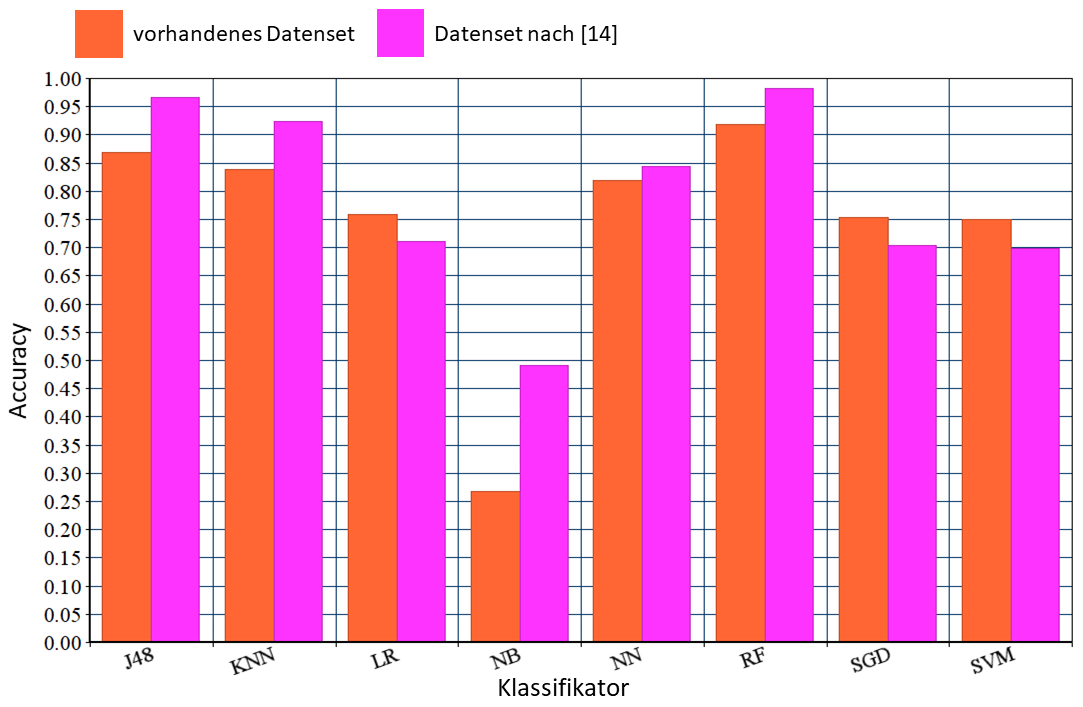
\includegraphics[width=\textwidth]{images/Klasseval}
    \caption{Übersicht der Accuracies des nicht-featurebasierten Vergleichs\label{fig:class-acc}}
\end{figure}

\begin{figure}
  \centering
  \subfloat[][J48 (vorh. Datenset)]{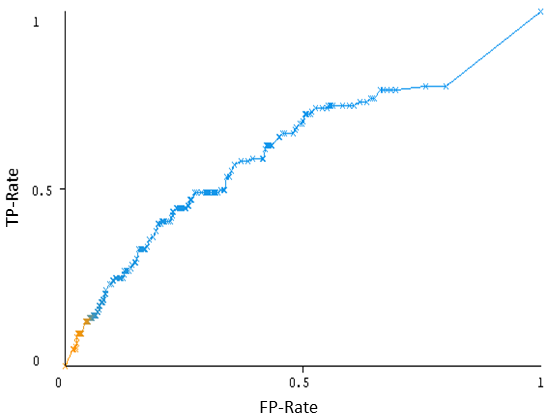
\includegraphics[width=0.25\linewidth]{images/j48_eval_feat}}
  \subfloat[][J48 nach \cite{Moser2008}]{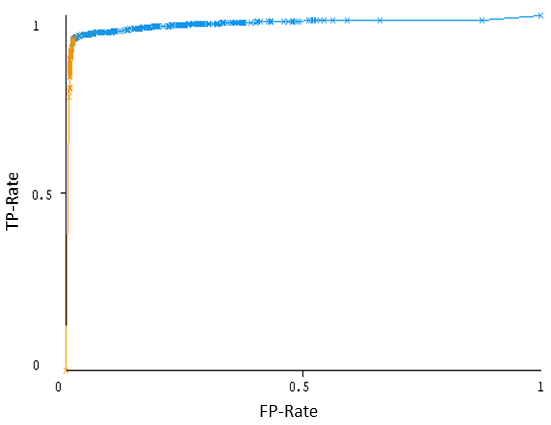
\includegraphics[width=0.25\linewidth]{images/j48_eval}}
  \subfloat[][NN (vorh. Datenset)]{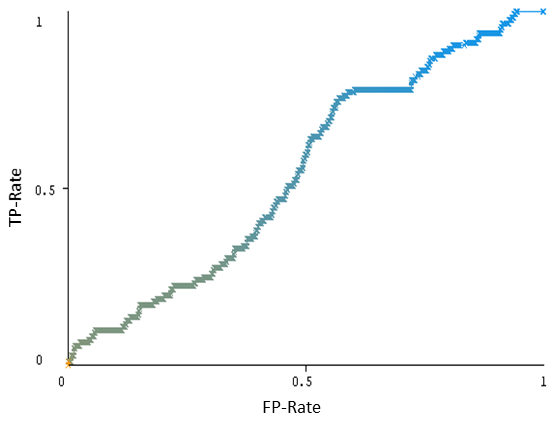
\includegraphics[width=0.25\linewidth]{images/nn_eval_feat}}
  \subfloat[][NN nach \cite{Moser2008}]{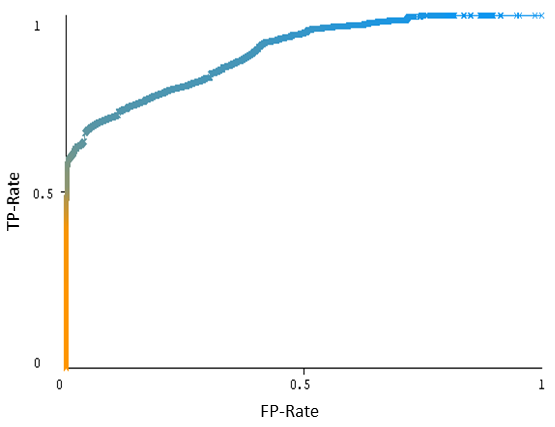
\includegraphics[width=0.25\linewidth]{images/nn_eval}}
  \qquad
  \subfloat[][KNN (vorh. Datenset)]{\includegraphics[width=0.25\linewidth]{images/knn_eval_feat}}
  \subfloat[][KNN nach \cite{Moser2008}]{\includegraphics[width=0.25\linewidth]{images/knn_eval}}
  \subfloat[][RF (vorh. Datenset)]{\includegraphics[width=0.25\linewidth]{images/rf_eval_feat}}
  \subfloat[][RF nach \cite{Moser2008}]{\includegraphics[width=0.25\linewidth]{images/rf_eval}}  
  \qquad
  \subfloat[][LR (vorh. Datenset)]{\includegraphics[width=0.25\linewidth]{images/lr_eval_feat}}
  \subfloat[][LR nach \cite{Moser2008}]{\includegraphics[width=0.25\linewidth]{images/lr_eval}}
  \subfloat[][SGD (vorh. Datenset)]{\includegraphics[width=0.25\linewidth]{images/sgd_eval_feat}}
  \subfloat[][SGD nach \cite{Moser2008}]{\includegraphics[width=0.25\linewidth]{images/sgd_eval}}
  \qquad
  \subfloat[][NB (vorh. Datenset)]{\includegraphics[width=0.25\linewidth]{images/nb_eval_feat}}
  \subfloat[][NB nach \cite{Moser2008}]{\includegraphics[width=0.25\linewidth]{images/nb_eval}}
  \subfloat[][SVM (vorh. Datenset)]{\includegraphics[width=0.25\linewidth]{images/svm_eval_feat}}
  \subfloat[][SVM nach \cite{Moser2008}]{\includegraphics[width=0.25\linewidth]{images/svm_eval}}
  \caption{ROC-Kurven des nicht-featurebasierten Vergleichs}
\end{figure}


\begin{table}[t]
\centering
\caption{Ergebnisse der Evaluationsmetriken des nicht-featurebasierten Vergleichs}
\label{tab:class-val}
\resizebox{\linewidth}{!}{%
\begin{tabular}{|>{\hspace{0pt}}p{0.083\linewidth}>{\hspace{0pt}}p{0.16\linewidth}|>{\RaggedLeft\hspace{0pt}}p{0.166\linewidth}>{\RaggedLeft\hspace{0pt}}p{0.108\linewidth}>{\RaggedLeft\hspace{0pt}}p{0.097\linewidth}|>{\RaggedLeft\hspace{0pt}}p{0.149\linewidth}>{\RaggedLeft\hspace{0pt}}p{0.108\linewidth}>{\RaggedLeft\hspace{0pt}}p{0.098\linewidth}|} 
\cline{3-8}
\multicolumn{1}{>{\hspace{0pt}}p{0.083\linewidth}}{}           &           & \multicolumn{3}{>{\Centering\hspace{0pt}}p{0.371\linewidth}|}{\textbf{Datenset nach \cite{Moser2008}} } & \multicolumn{3}{>{\Centering\hspace{0pt}}p{0.355\linewidth}|}{\textbf{vorhandenes Datenset}}  \\ 
\cline{3-8}
\multicolumn{1}{>{\Centering\hspace{0pt}}p{0.083\linewidth}}{} &           & \textbf{fehlerfrei}~~ & \textbf{defekt} & \textbf{gew.}\par{}\textbf{Mittel}           & \textbf{fehlerfrei}  & \textbf{defekt}  & \textbf{gew.}\par{}\textbf{Mittel}                  \\ 
\hline
\multirow{4}{0.083\linewidth}{\hspace{0pt}DT}                  & Precision & 0,97                  & 0,96            & 0,97                                         & 0,90                 & 0,76             & 0,87                                                \\
                                                               & Recall    & 0,98                  & 0,93            & 0,97                                         & 0,93                 & 0,70             & 0,87                                                \\
                                                               & F-Score   & 0,98                  & 0,95            & 0,97                                         & 0,91                 & 0,73             & 0,87                                                \\
                                                               & ROC-Area  & 0,97                  & 0,97            & 0,97                                         & 0,86                 & 0,86             & 0,86                                                \\ 
\hline
\multirow{4}{0.083\linewidth}{\hspace{0pt}KNN}                 & Precision & 0,93                  & 0,91            & 0,92                                         & 0,87                 & 0,71             & 0,83                                                \\
                                                               & Recall    & 0,96                  & 0,85            & 0,92                                         & 0,92                 & 0,61             & 0,84                                                \\
                                                               & F-Score   & 0,95                  & 0,88            & 0,92                                         & 0,90                 & 0,65             & 0,83                                                \\
                                                               & ROC-Area  & 0,93                  & 0,93            & 0,93                                         & 0,77                 & 0,77             & 0,77                                                \\ 
\hline
\multirow{4}{0.083\linewidth}{\hspace{0pt}LR}                  & Precision & 0,72                  & 0,64            & 0,69                                         & 0,76                 & 0,65             & 0,74                                                \\
                                                               & Recall    & 0,96                  & 0,18            & 0,71                                         & 0,99                 & 0,08             & 0,76                                                \\
                                                               & F-Score   & 0,82                  & 0,65            & 0,28                                         & 0,86                 & 0,15             & 0,68                                                \\
                                                               & ROC-Area  & 0,77                  & 0,77            & 0,77                                         & 0,73                 & 0,73             & 0,73                                                \\ 
\hline
\multirow{4}{0.083\linewidth}{\hspace{0pt}NB}                  & Precision & 0,90                  & 0,38            & 0,73                                         & 0,65                 & 0,26             & 0,55                                                \\
                                                               & Recall    & 0,29                  & 0,93            & 0,49                                         & 0,03                 & 0,96             & 0,27                                                \\
                                                               & F-Score   & 0,44                  & 0,54            & 0,47                                         & 0,05                 & 0,41             & 0,14                                                \\
                                                               & ROC-Area  & 0,73                  & 0,73            & 0,73                                         & 0,61                 & 0,61             & 0,61                                                \\ 
\hline
\multirow{4}{0.083\linewidth}{\hspace{0pt}NN}                  & Precision & 0,82                  & 0,99            & 0,87                                         & 0,83                 & 0,76             & 0,81                                                \\
                                                               & Recall    & 1,00                  & 0,51            & 0,84                                         & 0,86                 & 0,42             & 0,82                                                \\
                                                               & F-Score   & 0,90                  & 0,67            & 0,83                                         & 0,89                 & 0,54             & 0,80                                                \\
                                                               & ROC-Area  & 0,89                  & 0,89            & 0,89                                         & 0,85                 & 0,85             & 0,85                                                \\ 
\hline
\multirow{4}{0.083\linewidth}{\hspace{0pt}RF}                  & Precision & 0,98                  & 0,98            & 0,98                                         & 0,93                 & 0,88             & 0,92                                                \\
                                                               & Recall    & 0,99                  & 0,96            & 0,98                                         & 0,96                 & 0,79             & 0,92                                                \\
                                                               & F-Score   & 0,99                  & 0,97            & 0,98                                         & 0,95                 & 0,83             & 0,92                                                \\
                                                               & ROC-Area  & 1,00                  & 1,00            & 1,00                                         & 0,97                 & 0,97             & 0,97                                                \\ 
\hline
\multirow{4}{0.083\linewidth}{\hspace{0pt}SGD}                 & Precision & 0,71                  & 0,68            & 0,70                                         & 0,75                 & 0,78             & 0,76                                                \\
                                                               & Recall    & 0,98                  & 0,10            & 0,70                                         & 1,00                 & 0,02             & 0,75                                                \\
                                                               & F-Score   & 0,82                  & 0,18            & 0,62                                         & 0,86                 & 0,03             & 0,65                                                \\
                                                               & ROC-Area  & 0,54                  & 0,54            & 0,54                                         & 0,51                 & 0,51             & 0,51                                                \\ 
\hline
\multirow{4}{0.083\linewidth}{\hspace{0pt}SVM}                 & Precision & 0,70                  & 0,66            & 0,69                                         & 0,75                 & ?                & ?                                                   \\
                                                               & Recall    & 0,98                  & 0,07            & 0,70                                         & 1,00                 & 0,00             & 0,75                                                \\
                                                               & F-Score   & 0,82                  & 0,13            & 0,60                                         & 0,86                 & ?                & ?                                                   \\
                                                               & ROC-Area  & 0,53                  & 0,53            & 0,53                                         & 0,50                 & 0,50             & 0,50                                                \\
\hline
\end{tabular}
}
\end{table}

\cleardoublepage
